\documentclass[11pt,a4paper]{article}

\usepackage[margin=2.5cm]{geometry}
\usepackage{amsmath,amssymb}
\usepackage{graphicx}
\usepackage{booktabs}
\usepackage{siunitx}
\usepackage{hyperref}
\usepackage{xcolor}
\usepackage{microtype}

\hypersetup{
    colorlinks=true,
    linkcolor=blue,
    citecolor=blue,
    urlcolor=blue
}

\title{
    \textbf{CFD Mesh Refinement Using Self-Organizing Maps}\\[0.4cm]
    \large Evaluation of SOM-Based and Hybrid Refinement Indicators\\
    for the Lid-Driven Cavity
}

\author{
    José David Jiménez Díaz\\[0.15cm]
    \small Independent Engineering Research\\
    \small Mississauga, Ontario, Canada\\[0.1cm]
    \small \href{mailto:jd.jimenez.eng@gmail.com}{jd.jimenez.eng@gmail.com}\\
    \small \href{https://www.linkedin.com/in/josedavidjimenezdiazeng/}
    {linkedin.com/in/josedavidjimenezdiazeng}\\
    \small \href{https://github.com/JoseJimenezD/CFD-SOM-Adaptive-Meshing}
    {github.com/JoseJimenezD/CFD-SOM-Adaptive-Meshing}
}

\date{September 2026}

\begin{document}

\maketitle

\begin{abstract}
This technical report investigates whether information learned by a
Self-Organizing Map (SOM) can contribute to adaptive mesh-refinement
decisions in computational fluid dynamics. A two-dimensional lid-driven
cavity at Reynolds number \(Re=100\) is used as a controlled benchmark,
with a fine uniform M160 solution serving as a numerical reference for
post-solution evaluation.

The study first compares conventional velocity-gradient refinement with
direct refinement based on SOM quantization error (SOM-QE) and with a
hybrid gradient--SOM indicator under controlled refinement budgets.
Direct SOM-QE refinement does not outperform the conventional Gradient
criterion and exhibits non-monotonic behavior with increasing refinement
budget. This negative result motivates a reformulation of the role of the
SOM: rather than treating quantization error as a proxy for discretization
error, the SOM is used to identify spatial transitions between
SOM-classified flow states.

A SOM-interface indicator is subsequently constructed from BMU-state
transitions, local velocity-gradient magnitude, and velocity jumps across
neighboring SOM states. Using a fixed set of 40 priority seeds followed by
one- and two-neighbor expansion, the resulting adaptive meshes are compared
with Gradient meshes having matched final cell counts. For this cavity and
the tested configuration, SOM-interface produces lower mean and RMS
discrepancies relative to the M160 reference at both matched mesh sizes,
while Gradient produces slightly lower maximum discrepancies. These results
are therefore evidence for the tested configuration rather than a claim of
general superiority.

A controlled sensitivity study further evaluates SOM architectures from
\(3\times3\) to \(6\times6\), with five random initializations per
architecture. The density of SOM-state interfaces depends strongly on map
resolution, while exact top-40 seed selection also exhibits initialization
sensitivity. However, for the nominal \(4\times4\) SOM, mean spatial
agreement between seed sets increases from 66.5\% for exact cell matching
to 89.5\% within one base-grid cell and 96.0\% within two cells, indicating
that much of the initialization sensitivity corresponds to local shifts
rather than wholesale relocation of the selected regions.

The study demonstrates a reproducible workflow for separating SOM
representation quality from numerical refinement utility and for evaluating
machine-learning-derived mesh indicators without using the numerical
reference during cell selection. The conclusions remain limited to a
single laminar benchmark, one Reynolds number, and one-shot adaptive
refinement; broader CFD cases and repeated adaptation cycles are required
before assessing general applicability.
\end{abstract}

\tableofcontents
\newpage

\section{Introduction}

\section{CFD Model}
\label{sec:cfd_model}

\subsection{Benchmark problem}

The two-dimensional lid-driven cavity was selected as the initial benchmark
problem because it provides a simple geometry while producing a non-trivial
recirculating incompressible flow field. The problem has also been extensively
used for the verification and comparison of numerical methods. Classical
reference solutions and detailed analyses of this benchmark are available in
Ghia et al., Botella and Peyret, and Shankar and Deshpande
\cite{ghia1982,botella1998,shankar2000}.

The computational domain is a square cavity with characteristic length

\begin{equation}
L = 0.1~\mathrm{m}.
\end{equation}

The upper wall moves in the positive \(x\)-direction with constant velocity

\begin{equation}
U_{\mathrm{lid}} = 1~\mathrm{m\,s^{-1}},
\end{equation}

while the remaining cavity walls are stationary. The kinematic viscosity is

\begin{equation}
\nu = 1.0\times10^{-3}~\mathrm{m^2\,s^{-1}}.
\end{equation}

The corresponding Reynolds number is therefore

\begin{equation}
Re =
\frac{U_{\mathrm{lid}}L}{\nu}
=
100.
\end{equation}

Although the OpenFOAM computational mesh has a finite thickness in the
\(z\)-direction, the front and back boundaries are defined using the
\texttt{empty} boundary condition. The calculation therefore represents a
two-dimensional flow problem.

\subsection{Numerical solution}

The incompressible transient Navier--Stokes equations are solved using
OpenFOAM v2606. The \texttt{icoFoam} solver is used for the present benchmark.
The numerical formulation follows the finite-volume framework underlying
OpenFOAM; general finite-volume CFD methodology is described by Ferziger and
Peri\'c and by Versteeg and Malalasekera
\cite{weller1998,ferziger2002,versteeg2007,openfoam2606}.

The velocity field is denoted by \(\mathbf{U}\), and the pressure field by
\(p\). The governing equations are

\begin{equation}
\nabla\cdot\mathbf{U}=0,
\end{equation}

and

\begin{equation}
\frac{\partial\mathbf{U}}{\partial t}
+
(\mathbf{U}\cdot\nabla)\mathbf{U}
=
-\nabla p
+
\nu\nabla^2\mathbf{U}.
\end{equation}

The CFD solution obtained on the initial mesh provides the physical
information subsequently used to construct conventional and SOM-based
refinement indicators.

The machine-learning model therefore does not replace the governing
equations or the CFD solver. Instead, it operates on quantities extracted
from a physics-based CFD solution.


\section{Numerical Verification}
\label{sec:verification}

Before evaluating machine-learning-based refinement strategies, a uniform-mesh
refinement study was performed to establish the numerical behavior of the
baseline CFD model. Grid-refinement studies and observed-order analyses are
standard components of CFD solution verification
\cite{roache1998,celik2008}.

Four structured meshes were considered, denoted M20, M40, M80, and M160.
Successive refinement approximately halves the characteristic cell spacing
in each coordinate direction.

\begin{table}[htbp]
\centering
\caption{Uniform meshes used for the numerical verification study.}
\label{tab:uniform_meshes}
\begin{tabular}{lrrr}
\toprule
Mesh & Cells & $\Delta x$ [m] & Minimum $U_x/U_{\mathrm{lid}}$ \\
\midrule
M20  & 400    & 0.00500 & -0.198089 \\
M40  & 1600   & 0.00250 & -0.209591 \\
M80  & 6400   & 0.00125 & -0.212887 \\
M160 & 25600  & 0.000625 & -0.213733 \\
\bottomrule
\end{tabular}
\end{table}

A vertical velocity sampling line located at the horizontal center of the
cavity,

\begin{equation}
x/L = 0.5,
\end{equation}

was used to compare the horizontal velocity component between successive
meshes.

The resulting inter-grid differences are summarized in
Table~\ref{tab:grid_convergence}.

\begin{table}[htbp]
\centering
\caption{Successive-mesh differences for the vertical centerline velocity
profile.}
\label{tab:grid_convergence}
\begin{tabular}{lrr}
\toprule
Mesh comparison & $L_2$ difference & $L_\infty$ difference \\
\midrule
M20--M40   & $6.1826\times10^{-3}$ & $1.2598\times10^{-2}$ \\
M40--M80   & $1.7211\times10^{-3}$ & $3.5090\times10^{-3}$ \\
M80--M160  & $4.2841\times10^{-4}$ & $8.8600\times10^{-4}$ \\
\bottomrule
\end{tabular}
\end{table}

The reduction ratios of the successive \(L_2\) differences are approximately

\begin{equation}
\frac{E_{20,40}}{E_{40,80}} = 3.59,
\qquad
\frac{E_{40,80}}{E_{80,160}} = 4.02.
\end{equation}

For a refinement ratio of approximately two, an observed convergence order
can be estimated from the successive solution differences, consistent with
standard grid-refinement verification practice
\cite{roache1998,celik2008}:

\begin{equation}
p =
\frac{\ln(E_h/E_{h/2})}{\ln(2)}.
\end{equation}

The corresponding observed orders are approximately

\begin{equation}
p = 1.845
\end{equation}

for the M20--M40--M80 sequence and

\begin{equation}
p = 2.006
\end{equation}

for the M40--M80--M160 sequence.

These results indicate strong convergence of the sampled centerline velocity
profile, with behavior approaching second order on the finer meshes.

\subsection{Reference solution used in the adaptive-mesh study}

The M160 solution is subsequently used as a fine-grid numerical reference
for comparisons with the adaptive meshes. It is important to emphasize that
M160 is not treated as an exact analytical solution or as a formally
grid-independent solution.

Consequently, quantities reported later as ``error'' relative to M160 should
more precisely be interpreted as discrepancies with respect to the selected
fine-grid numerical reference.

\subsection{Verification limitations}

The time step was reduced together with the spatial mesh size during the
uniform refinement sequence. Therefore, the present refinement study does
not rigorously separate spatial discretization error from temporal
discretization effects.

Furthermore, the discontinuity between the moving lid and the stationary
side walls produces strong gradients near the upper corners of the cavity.
These regions can dominate pointwise error measures and must be considered
carefully when interpreting maximum-error metrics.

For these reasons, the verification study is used to establish numerical
consistency and to define a controlled internal reference for the subsequent
comparisons, rather than to claim an exact discretization-error estimate.


\section{Self-Organizing Map Methodology}
\label{sec:som_methodology}

\subsection{Purpose of the SOM}

A Self-Organizing Map (SOM) was introduced to investigate whether
unsupervised learning could identify physically meaningful flow states in the
CFD solution and whether information derived from those states could
subsequently contribute to mesh-refinement decisions.

The SOM is an unsupervised neural-network method that maps multidimensional
input data onto a lower-dimensional discrete lattice while attempting to
preserve topological relationships in the input space
\cite{kohonen1982,kohonen2001}. SOM-based clustering and interpretation of
the trained map have subsequently been developed for exploratory analysis of
multidimensional data \cite{vesanto2000}.

In the present work, the SOM is not used as a surrogate for the CFD solver.
The Navier--Stokes equations remain the source of the physical solution.
Instead, the SOM analyzes quantities extracted from the CFD field.

The initial SOM analysis is performed using the M40 solution, containing
1600 cells. Importantly, the M160 reference solution is not used during SOM
training or during the construction of the refinement indicators. It is
reserved for subsequent evaluation.

The supporting data-analysis workflow was implemented in Python using the
scientific-computing ecosystem. Array and numerical operations relied on
NumPy and SciPy, while preprocessing utilities were drawn from
scikit-learn \cite{harris2020,virtanen2020,pedregosa2011}.

\subsection{Candidate physical features}

For each M40 cell, the CFD post-processing pipeline extracts the cell-center
coordinates and local flow quantities. The candidate nondimensional
quantities include

\begin{equation}
\frac{U_x}{U_{\mathrm{lid}}},
\qquad
\frac{U_y}{U_{\mathrm{lid}}},
\qquad
\frac{|\mathbf{U}|}{U_{\mathrm{lid}}},
\qquad
\frac{L|\nabla\mathbf{U}|}{U_{\mathrm{lid}}},
\qquad
\frac{L|\boldsymbol{\omega}|}{U_{\mathrm{lid}}},
\end{equation}

where

\begin{equation}
\boldsymbol{\omega}=\nabla\times\mathbf{U}.
\end{equation}

The velocity-gradient magnitude is computed using the Frobenius norm of the
velocity-gradient tensor.

Spatial coordinates are deliberately excluded from the SOM input vector.
Consequently, any spatially coherent classification produced by the SOM must
arise from similarities in the local flow state rather than from explicit
knowledge of cell position.

\subsection{Feature selection}

An exploratory correlation analysis showed a strong correlation between the
velocity-gradient magnitude and the vorticity magnitude,

\begin{equation}
r\left(|\nabla\mathbf{U}|,|\boldsymbol{\omega}|\right)
=
0.981.
\end{equation}

To reduce this strong redundancy, vorticity was excluded from the first SOM
input vector.

The resulting feature vector was

\begin{equation}
\mathbf{x}_i =
\begin{bmatrix}
U_{x,i}^{*} &
U_{y,i}^{*} &
|\mathbf{U}_i|^{*} &
|\nabla\mathbf{U}_i|^{*}
\end{bmatrix}^{T},
\end{equation}

where the superscript \(^{*}\) denotes physical nondimensionalization using
the characteristic cavity length and lid velocity.

The velocity magnitude is mathematically related to its two velocity
components and therefore introduces some redundancy. It was retained in this
initial investigation to preserve an explicit scalar measure of local flow
speed. Feature-ablation studies are left for future work.

\subsection{Standardization}

Physical nondimensionalization and machine-learning standardization are
treated as separate operations.

After nondimensionalization, each SOM feature is standardized according to

\begin{equation}
z_j =
\frac{x_j-\mu_j}{\sigma_j},
\end{equation}

where \(\mu_j\) and \(\sigma_j\) are respectively the mean and standard
deviation of feature \(j\) over the M40 dataset.

This prevents variables with larger numerical ranges from dominating the
Euclidean distance used during SOM training.

\subsection{SOM architecture and training}

The SOM consists of a \(4\times4\) rectangular lattice containing 16 neurons.
The implementation was developed in Python using NumPy, with feature
standardization performed using \texttt{StandardScaler}.

Training used 20,000 iterations with a fixed random seed of 42 to provide
reproducibility. The learning rate decreased exponentially from

\begin{equation}
\alpha_0=0.5
\end{equation}

to

\begin{equation}
\alpha_f=0.05,
\end{equation}

while the neighborhood radius decreased from

\begin{equation}
\sigma_0=2.0
\end{equation}

to

\begin{equation}
\sigma_f=0.5.
\end{equation}

A Gaussian neighborhood function was used during weight updates.

For each CFD cell, the best-matching unit (BMU) is the neuron whose weight
vector has the smallest Euclidean distance to the standardized feature
vector.

\subsection{Quantization error}

The cell-level SOM quantization error is defined as

\begin{equation}
QE_i =
\left\|
\mathbf{z}_i-\mathbf{w}_{b(i)}
\right\|_2,
\end{equation}

where \(\mathbf{z}_i\) is the standardized feature vector of cell \(i\) and
\(\mathbf{w}_{b(i)}\) is the weight vector of its BMU.

For the trained M40 SOM, the mean cell-level quantization error was

\begin{equation}
\overline{QE}=0.4976,
\end{equation}

while the maximum value was

\begin{equation}
QE_{\max}=7.5142.
\end{equation}

All 16 neurons contained assigned CFD cells after training.

A large quantization error indicates that a CFD state is represented
relatively poorly by its assigned SOM neuron. It does not, by definition,
represent CFD discretization error. Distinguishing these two quantities is
central to the experiments presented later in this report.

\subsection{Interpretation of SOM states}

Despite the exclusion of the spatial coordinates from the training features,
the resulting BMU assignments form spatially coherent regions when mapped
back onto the cavity.

This observation indicates that the SOM is identifying recurring local flow
states rather than arbitrary spatial locations. Different neurons represent
combinations of velocity direction, velocity magnitude, and velocity-gradient
magnitude.

The SOM therefore provides a classification of the local physical state.
Whether this classification contains information useful for adaptive
refinement is treated as an experimental question rather than an assumption.


\section{Adaptive Mesh Refinement Methodology}
\label{sec:adaptive_refinement}

Adaptive mesh refinement is a well-established strategy for concentrating
computational resolution in selected regions of a numerical domain. Classical
AMR methods provide important historical context for the general concept of
local refinement \cite{berger1984,berger1989}. The cell-selection indicators
developed in the present work are not implementations of those classical AMR
algorithms; they constitute a separate one-shot refinement experiment built
around the OpenFOAM solution and the SOM-derived information.

\subsection{Controlled comparison}

Three cell-selection strategies were evaluated under identical refinement
budgets:

\begin{enumerate}
    \item a conventional velocity-gradient indicator;
    \item direct refinement based on SOM quantization error (SOM-QE);
    \item a hybrid indicator combining the velocity gradient with
    SOM-derived regime-transition information.
\end{enumerate}

For each method, refinement budgets of 5\%, 10\%, 15\%, and 20\% of the
1600-cell M40 baseline mesh were considered.

The corresponding numbers of initially selected cells were therefore 80,
160, 240, and 320 cells, respectively.

The same local refinement operation was applied after cell selection.
Consequently, the final adaptive meshes contained 1840, 2080, 2320, and
2560 cells for the four refinement budgets.

This design isolates the effect of the cell-selection criterion: at a given
budget, each method starts from the same M40 solution, selects the same
number of cells, and uses the same refinement procedure.

\subsection{Velocity-gradient indicator}

The conventional baseline ranks cells according to the local velocity-gradient
magnitude,

\begin{equation}
G_i = |\nabla\mathbf{U}_i|.
\end{equation}

Cells with the largest values of \(G_i\) are selected until the prescribed
refinement budget is reached.

This method provides a physically interpretable conventional baseline:
regions in which the velocity field varies rapidly receive higher refinement
priority.

\subsection{Direct SOM quantization-error indicator}

The first SOM-based hypothesis uses the cell-level quantization error directly
as a refinement indicator,

\begin{equation}
I_{\mathrm{QE},i}=QE_i.
\end{equation}

Cells with the largest quantization errors are selected first.

This criterion tests whether CFD states that are poorly represented by the
trained SOM also correspond to locations where additional spatial resolution
is beneficial.

No fine-grid reference information is used during this selection.

\subsection{SOM regime-transition indicator}

The BMU classification provides a discrete label \(b_i\) for every M40 cell.
To identify interfaces between different SOM-classified flow states, a local
transition indicator is defined using the direct structured-grid neighbors of
cell \(i\):

\begin{equation}
T_i =
\frac{
\displaystyle
\sum_{j\in\mathcal{N}_i}
\mathbb{I}(b_j\neq b_i)
}{
|\mathcal{N}_i|
},
\end{equation}

where \(\mathcal{N}_i\) is the set of existing direct neighbors and
\(\mathbb{I}\) is the indicator function.

Thus,

\begin{equation}
0\leq T_i\leq1.
\end{equation}

A value of zero indicates that all direct neighbors belong to the same SOM
state, while larger values indicate increasing local interaction between
different SOM-classified states.

The transition indicator is constructed exclusively from the M40 SOM
classification. It does not use the M160 reference solution.

The cell-level correlation between the transition indicator and the
velocity-gradient magnitude was approximately

\begin{equation}
r(G,T)=0.261,
\end{equation}

substantially smaller than the correlation between gradient magnitude and
quantization error,

\begin{equation}
r(G,QE)=0.879.
\end{equation}

The transition indicator therefore contains information that is less
redundant with the conventional gradient criterion than the direct
quantization error.

\subsection{Hybrid-v1 indicator}

The hybrid indicator was designed to preserve the conventional gradient as
the primary refinement signal while allowing SOM regime-transition
information to modify the ranking of cells.

The normalized gradient is defined as

\begin{equation}
G_i^{*} =
\frac{G_i}{\max_j G_j}.
\end{equation}

The Hybrid-v1 indicator is then

\begin{equation}
I_{\mathrm{hyb},i}
=
G_i^{*}
\left(1+\alpha T_i\right),
\end{equation}

with

\begin{equation}
\alpha=0.5.
\end{equation}

The coefficient was fixed for the Hybrid-v1 experiment and was not optimized
against the M160 reference.

This distinction is important because tuning the coefficient to minimize
M160 discrepancies and subsequently evaluating performance against the same
M160 solution would contaminate the validation comparison.

Hybrid-v1 should therefore be interpreted as a predefined exploratory
indicator rather than an optimized model.

\subsection{Selection overlap}

Because the gradient remains the dominant component of Hybrid-v1, the hybrid
criterion modifies only a relatively small fraction of the conventional
gradient selections.

The overlap between Gradient and Hybrid-v1 selections was

\begin{table}[htbp]
\centering
\caption{Overlap between Gradient and Hybrid-v1 cell selections.}
\label{tab:gradient_hybrid_overlap}
\begin{tabular}{rrrrr}
\toprule
Budget & Selected & Common & Exclusive per method & Overlap \\
\midrule
5\%  & 80  & 73  & 7  & 91.25\% \\
10\% & 160 & 149 & 11 & 93.12\% \\
15\% & 240 & 227 & 13 & 94.58\% \\
20\% & 320 & 306 & 14 & 95.62\% \\
\bottomrule
\end{tabular}
\end{table}

Consequently, Hybrid-v1 is not a replacement of the gradient criterion by a
machine-learning criterion. It is a controlled perturbation of the
gradient-based ranking using information extracted from SOM flow-state
boundaries.


\subsection{Second-stage SOM-interface refinement criterion}

The results obtained with direct SOM quantization error motivated a change in
the evaluation question. Rather than treating the SOM as a direct estimator
of discretization error, the subsequent analysis asked whether the SOM
classification contains information about \emph{where refinement is likely to
be useful}.

The BMU field provides a spatial classification of local flow states. Cells
located at interfaces between different BMU states were therefore considered
potentially informative because they represent locations where the local flow
regime changes in the SOM feature space.

For an interface cell, the local transition fraction \(T_i\) was combined
with two quantities already available from the M40 pilot solution. The first
was the normalized velocity-gradient magnitude,

\begin{equation}
G_i^* =
\frac{G_i}{\max_j G_j},
\end{equation}

and the second was the normalized maximum velocity-vector jump across a
direct SOM interface,

\begin{equation}
\Delta U_i^* =
\frac{
\max_{j\in\mathcal{N}_i,\;b_j\neq b_i}
\|\mathbf{U}_i-\mathbf{U}_j\|_2
}{
\max_k \Delta U_k
}.
\end{equation}

The resulting SOM-interface ranking was defined as

\begin{equation}
I_{\mathrm{SI},i}
=
T_i
\sqrt{G_i^*\,\Delta U_i^*}.
\end{equation}

Only cells for which \(T_i>0\) were eligible for interface selection. The
highest-ranked 40 interface cells were then frozen as common seeds. Starting
from exactly those same seeds, the selected refinement region was expanded by
a fixed graph distance: one face-sharing layer for the \(1N\) case and two
layers for the \(2N\) case.

This construction deliberately separates two questions. The SOM determines
\emph{where flow-state transitions occur}, while the gradient and
velocity-jump terms determine how strongly those transitions are ranked.
Neither the M160 solution nor any reference-derived error field is used in
this construction.

The resulting experiments selected 78 cells for \(1N\) and 114 cells for
\(2N\). These counts were not forced to equal a nominal 10\% budget.
Instead, they were subsequently reproduced exactly with conventional
Gradient selection, creating cell-matched controls with identical final
cell counts. This comparison isolates the spatial-selection mechanism while
avoiding a confounding difference in total mesh size.

\subsection{Evaluation against the fine-grid reference}

After refinement, each adaptive case is solved independently with OpenFOAM.
The resulting velocity field is compared with the M160 fine-grid numerical
reference.

Because the adaptive and reference meshes contain different cell-center
locations, the M160 solution is interpolated to the adaptive-mesh cell
centers before the velocity discrepancy is evaluated.

For cell \(i\), the nondimensional velocity-vector discrepancy is

\begin{equation}
e_i =
\frac{
\left\|
\mathbf{U}_{i,\mathrm{adaptive}}
-
\mathbf{U}_{i,\mathrm{M160}}
\right\|_2
}{
U_{\mathrm{lid}}
}.
\end{equation}

Since adaptive cells have different volumes, global mean and RMS measures are
volume weighted.

The M160 solution is used only at this evaluation stage and not during the
selection of cells for Gradient, SOM-QE, or Hybrid-v1.


\section{Results}
\label{sec:results}

\subsection{Controlled adaptive-refinement matrix}

The three refinement strategies were evaluated at four identical refinement
budgets, producing a controlled matrix of 12 adaptive CFD simulations.
Table~\ref{tab:adaptive_results} summarizes the principal results.

\begin{table}[htbp]
\centering
\caption{Adaptive-mesh results relative to the M160 fine-grid numerical
reference. Mean and RMS velocity discrepancies are volume weighted. CPU time
corresponds to the final CFD solve and does not include the complete adaptive
workflow cost.}
\label{tab:adaptive_results}
\small
\begin{tabular}{llrrrr}
\toprule
Method & Budget & Cells & CPU [s] & Mean error & RMS error \\
\midrule
Gradient & 5\%  & 1840 & 9.64  & 0.001846 & 0.003994 \\
Gradient & 10\% & 2080 & 11.64 & 0.001656 & 0.003756 \\
Gradient & 15\% & 2320 & 13.62 & 0.001296 & 0.003505 \\
Gradient & 20\% & 2560 & 14.05 & 0.001105 & 0.003384 \\
\midrule
SOM-QE & 5\%  & 1840 & 9.62  & 0.002349 & 0.004392 \\
SOM-QE & 10\% & 2080 & 11.24 & 0.002628 & 0.004492 \\
SOM-QE & 15\% & 2320 & 12.53 & 0.002291 & 0.004175 \\
SOM-QE & 20\% & 2560 & 13.77 & 0.002005 & 0.003924 \\
\midrule
Hybrid-v1 & 5\%  & 1840 & 9.32  & 0.001841 & 0.004031 \\
Hybrid-v1 & 10\% & 2080 & 11.09 & 0.001583 & 0.003709 \\
Hybrid-v1 & 15\% & 2320 & 12.50 & 0.001394 & 0.003556 \\
Hybrid-v1 & 20\% & 2560 & 14.68 & 0.001242 & 0.003453 \\
\bottomrule
\end{tabular}
\end{table}

All adaptive meshes passed the mesh-quality checks used in the automated
experiment framework. The maximum Courant number remained below the imposed
limit of 1.05 for all cases.

\subsection{RMS discrepancy}

Figure~\ref{fig:rms_cells} compares the volume-weighted RMS velocity
discrepancy as a function of final adaptive-mesh cell count.

\begin{figure}[htbp]
\centering
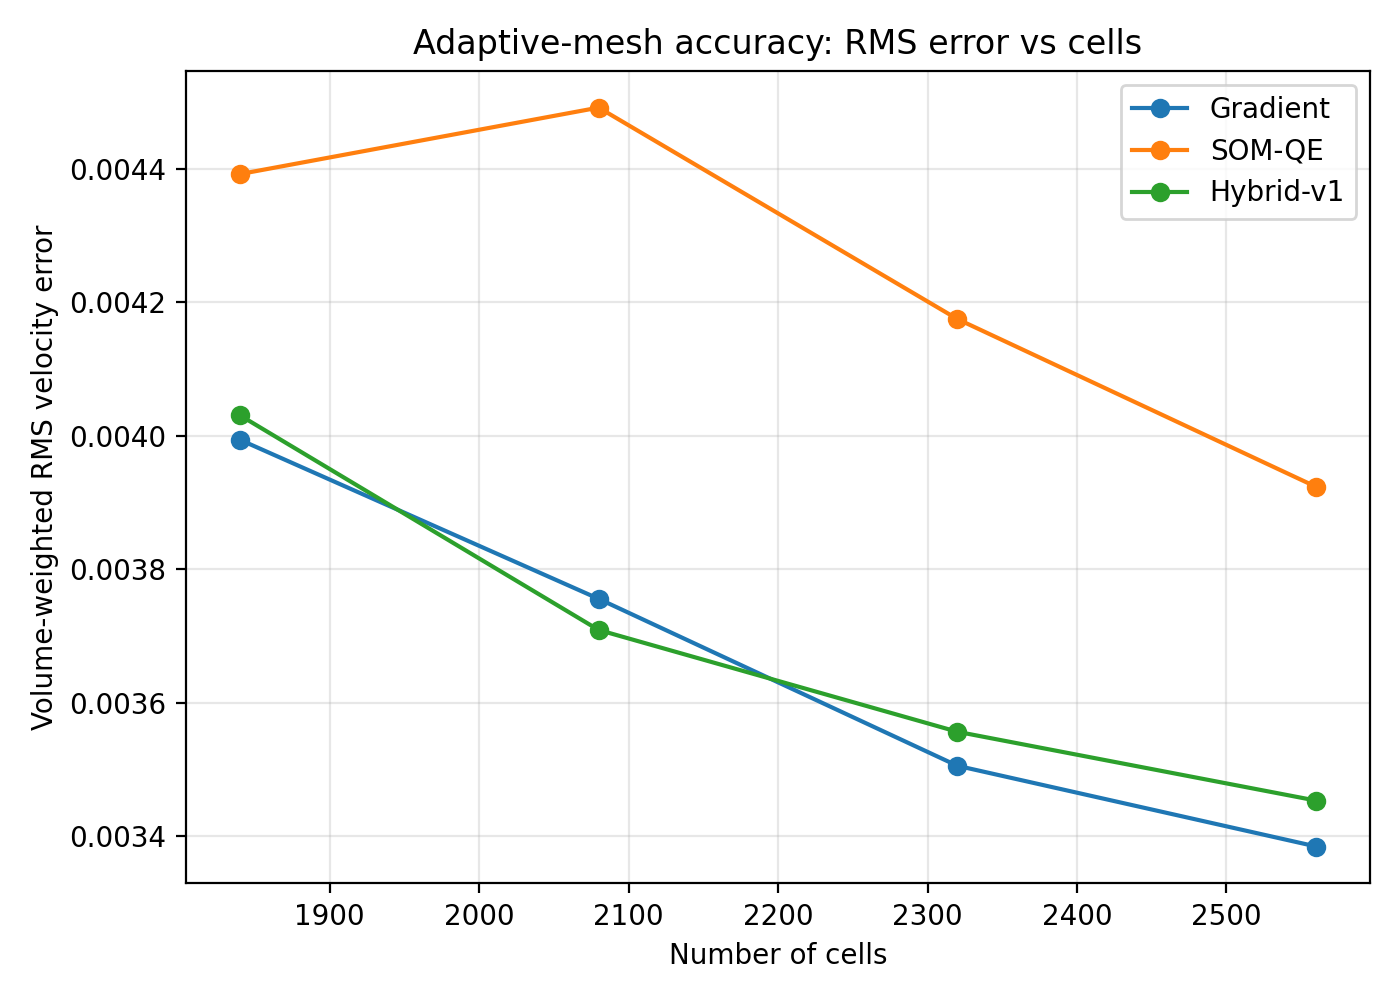
\includegraphics[width=0.88\textwidth]
{figures/RMS_vs_cells_3methods.png}
\caption{Volume-weighted RMS velocity discrepancy relative to the M160
fine-grid numerical reference for Gradient, SOM-QE, and Hybrid-v1 refinement.}
\label{fig:rms_cells}
\end{figure}

The Gradient criterion exhibits monotonic improvement as the refinement
budget increases. Its RMS discrepancy decreases from approximately
\(3.994\times10^{-3}\) at the 5\% budget to
\(3.384\times10^{-3}\) at the 20\% budget.

Direct SOM-QE refinement does not exhibit the same behavior. In particular,
increasing the budget from 5\% to 10\% increases the RMS discrepancy from

\begin{equation}
4.392\times10^{-3}
\end{equation}

to

\begin{equation}
4.492\times10^{-3}.
\end{equation}

The SOM-QE criterion subsequently improves at the 15\% and 20\% budgets, but
its RMS discrepancy remains higher than that of Gradient at every tested
budget.

At equal refinement budgets, the Gradient RMS discrepancy is lower than the
SOM-QE result by approximately 9.1\%, 16.4\%, 16.0\%, and 13.7\% for the
5\%, 10\%, 15\%, and 20\% budgets, respectively.

These results do not support the hypothesis that SOM quantization error can
be used directly as a superior refinement indicator for the present cavity
problem.

\subsection{Hybrid-v1 performance}

Hybrid-v1 recovers monotonic RMS improvement with increasing refinement
budget and remains close to the Gradient baseline.

Relative to Gradient, the Hybrid-v1 RMS discrepancy changes by approximately

\begin{equation}
-0.92\%,\quad
+1.24\%,\quad
-1.45\%,\quad
-2.03\%
\end{equation}

at the 5\%, 10\%, 15\%, and 20\% budgets, respectively, where a positive
value denotes an improvement relative to Gradient.

Thus, Hybrid-v1 produces a small RMS improvement at the 10\% budget, but this
improvement is not reproduced at the other tested budgets. The present
results therefore do not demonstrate a systematic accuracy advantage of
Hybrid-v1 over the conventional Gradient criterion.

\subsection{Mean velocity discrepancy}

Figure~\ref{fig:mean_cells} presents the corresponding volume-weighted mean
velocity discrepancy.

\begin{figure}[htbp]
\centering
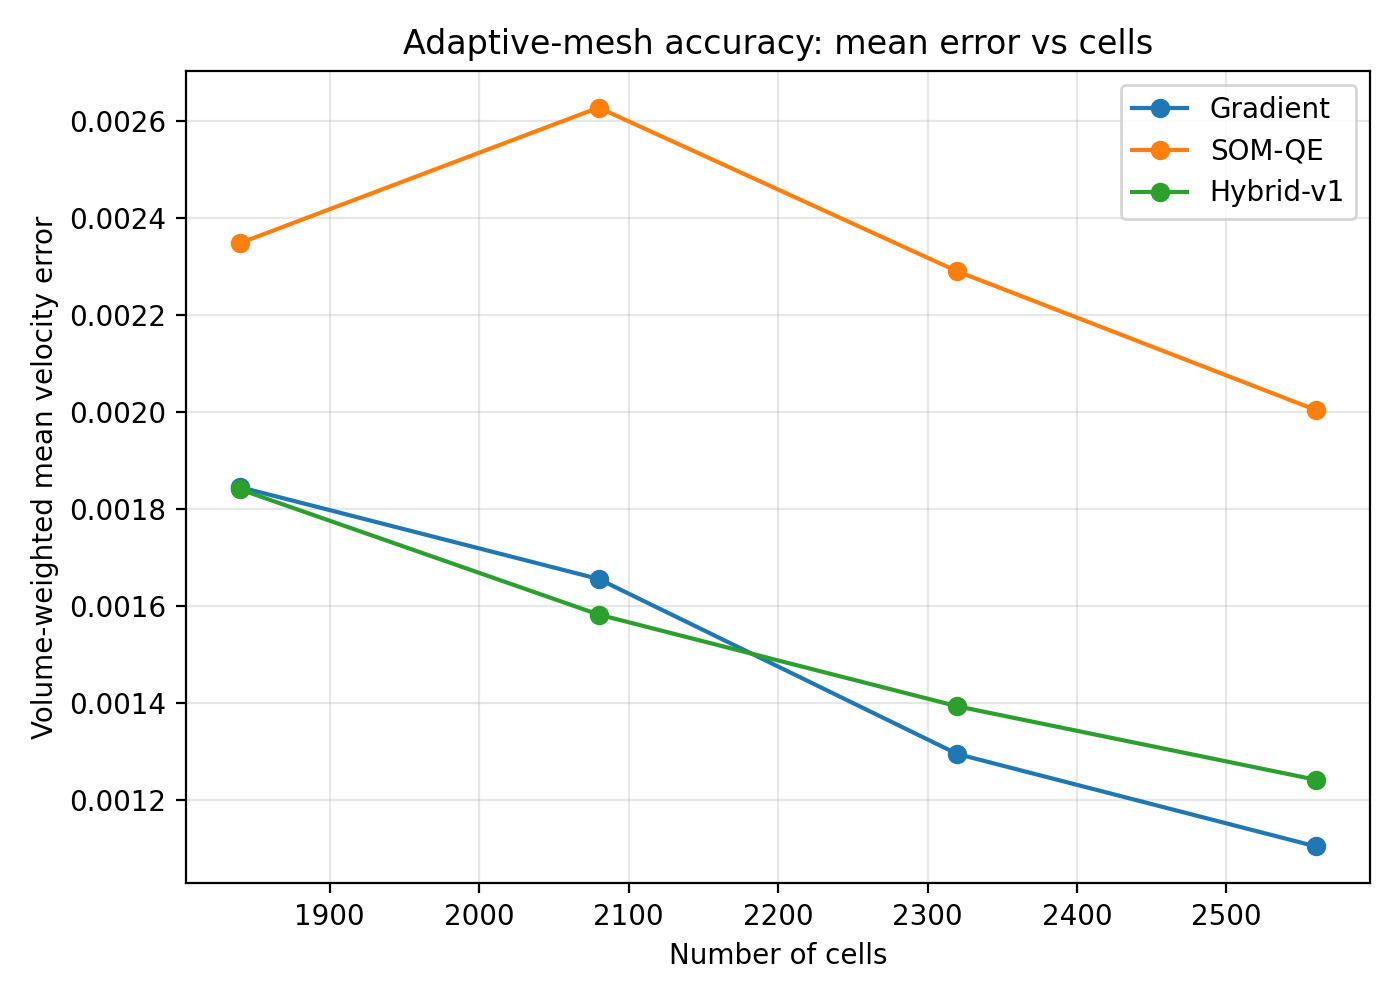
\includegraphics[width=0.88\textwidth]
{figures/Mean_vs_cells_3methods.png}
\caption{Volume-weighted mean velocity discrepancy relative to the M160
fine-grid numerical reference for the three refinement strategies.}
\label{fig:mean_cells}
\end{figure}

The mean-error results reinforce the RMS comparison. Gradient improves
monotonically from approximately \(1.846\times10^{-3}\) to
\(1.105\times10^{-3}\).

SOM-QE again exhibits non-monotonic behavior between the 5\% and 10\%
budgets. At the four tested budgets, the Gradient mean discrepancy is
approximately 21.4\%, 37.0\%, 43.4\%, and 44.9\% lower than the corresponding
SOM-QE result.

Hybrid-v1 produces a mean-error improvement of approximately 0.25\% and
4.43\% relative to Gradient at the 5\% and 10\% budgets, respectively.
However, at 15\% and 20\% its mean discrepancy is approximately 7.59\% and
12.44\% higher than Gradient.

As with the RMS metric, the hybrid modification therefore does not provide a
consistent advantage across refinement budgets.

\subsection{What Hybrid-v1 changes}

Because Hybrid-v1 preserves the gradient as its primary signal, its cell
selection remains strongly overlapping with the conventional Gradient
selection.

Figure~\ref{fig:gradient_hybrid_selection} shows the spatial distribution of
common and exclusive selections at all four budgets.

\begin{figure}[htbp]
\centering
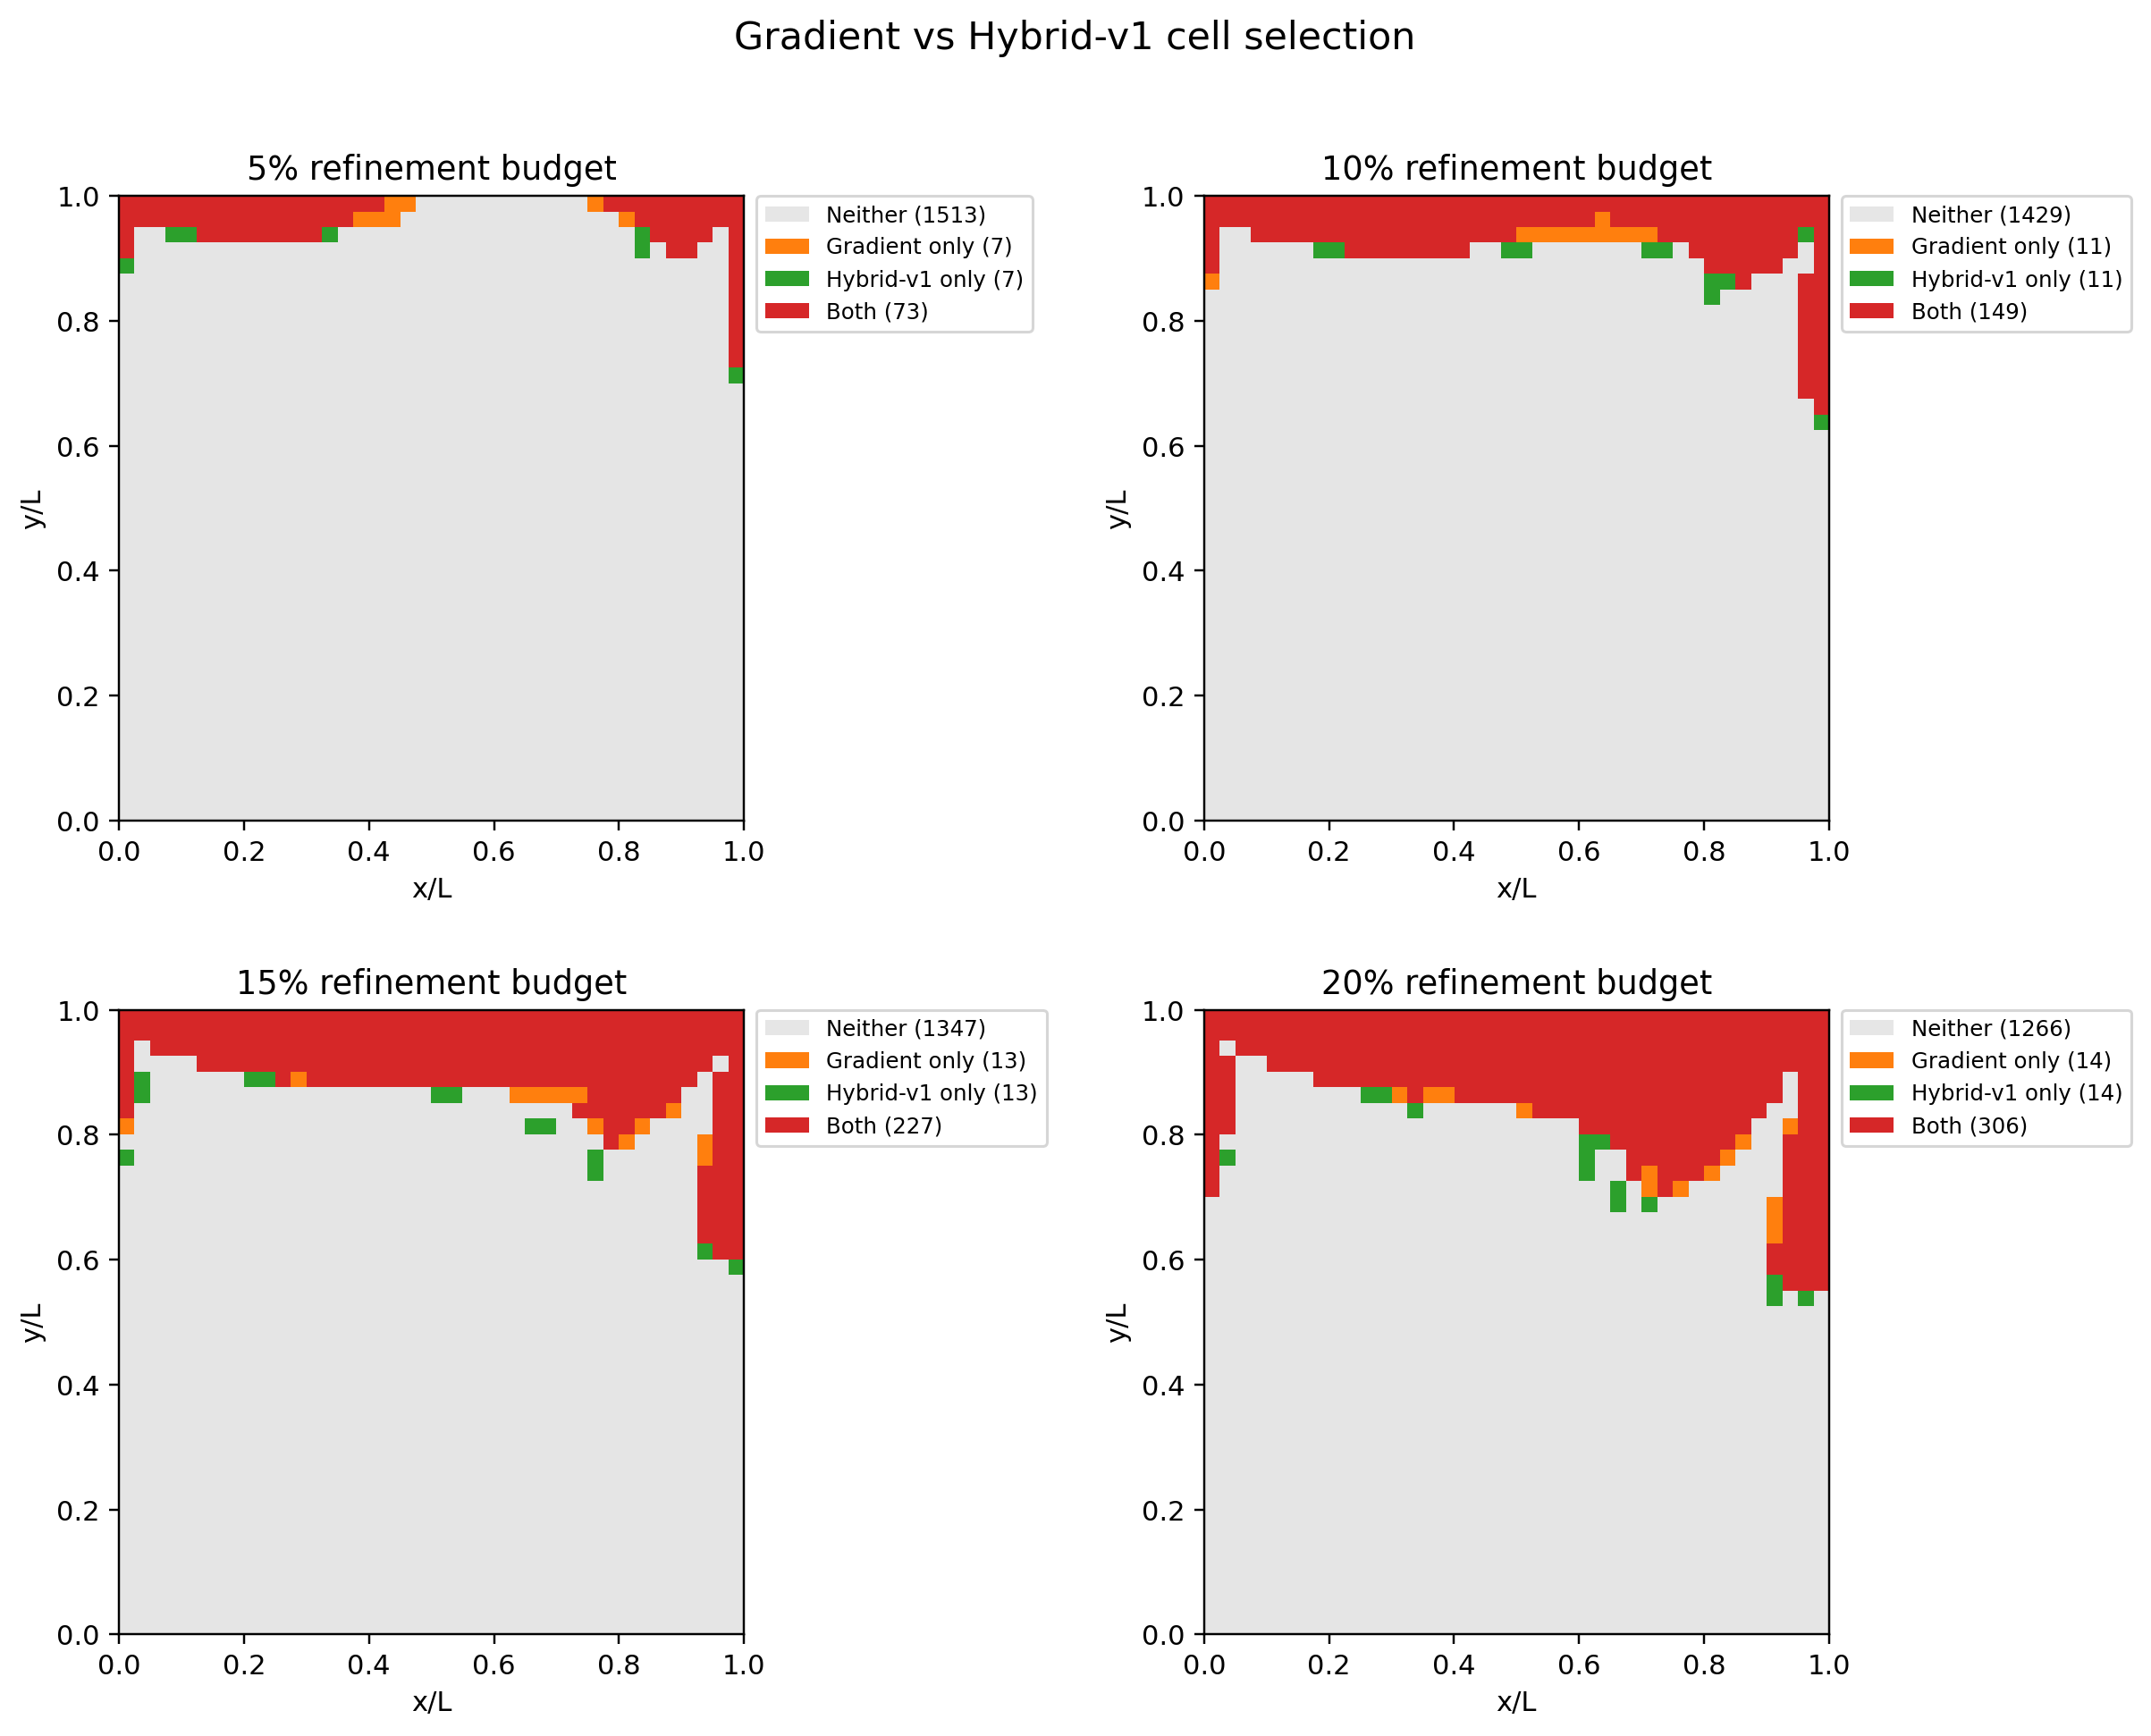
\includegraphics[width=0.98\textwidth]
{figures/Gradient_vs_Hybrid_selection_all_budgets.png}
\caption{Comparison of Gradient and Hybrid-v1 cell selections for refinement
budgets of 5\%, 10\%, 15\%, and 20\%. The hybrid formulation changes only a
small subset of cells close to the selection threshold.}
\label{fig:gradient_hybrid_selection}
\end{figure}

The overlap increases from 91.25\% at the 5\% budget to 95.62\% at the
20\% budget. Hybrid-v1 therefore acts as a controlled modification of the
Gradient ranking rather than as an independent replacement criterion.

To identify the physical nature of these changes, the cells selected
exclusively by each method were analyzed using only quantities available from
the M40 pilot solution. Table~\ref{tab:swap_statistics} summarizes the
results.

\begin{table}[htbp]
\centering
\caption{Mean characteristics of cells selected exclusively by Gradient or
Hybrid-v1. The analysis uses only M40 quantities and does not use the M160
reference.}
\label{tab:swap_statistics}
\small
\begin{tabular}{llrrr}
\toprule
Budget & Exclusive selection & Cells &
Mean $|\nabla U|^{*}$ & Mean $T$ \\
\midrule
5\%  & Gradient  & 7  & 7.489 & 0.000 \\
5\%  & Hybrid-v1 & 7  & 6.663 & 0.619 \\
10\% & Gradient  & 11 & 5.384 & 0.000 \\
10\% & Hybrid-v1 & 11 & 4.810 & 0.583 \\
15\% & Gradient  & 13 & 3.730 & 0.000 \\
15\% & Hybrid-v1 & 13 & 3.261 & 0.596 \\
20\% & Gradient  & 14 & 2.836 & 0.054 \\
20\% & Hybrid-v1 & 14 & 2.461 & 0.643 \\
\bottomrule
\end{tabular}
\end{table}

A consistent pattern is observed at all four budgets. Hybrid-v1 removes a
small number of cells having somewhat larger velocity gradients but little or
no SOM regime-transition activity and replaces them with cells having
slightly smaller gradients but substantially larger transition indicators.

For example, at the 10\% budget the Gradient-only cells have mean values

\begin{equation}
|\nabla U|^{*}=5.384,
\qquad
T=0,
\end{equation}

whereas the Hybrid-only cells have

\begin{equation}
|\nabla U|^{*}=4.810,
\qquad
T=0.583.
\end{equation}

The hybrid formulation is therefore behaving according to its intended
design: SOM information changes the priority of cells located near boundaries
between SOM-classified flow regimes.

However, the adaptive CFD results demonstrate that this physically
interpretable modification is not systematically beneficial. The 10\% case
improves the RMS discrepancy, whereas the same mechanism slightly worsens the
RMS result at 5\%, 15\%, and 20\%.

This distinction motivates a central result of the present investigation:
information that identifies a physically distinct flow state or a boundary
between states is not necessarily equivalent to information that predicts
the numerical utility of refining that location.

\subsection{Computational-time observations}

The measured solver execution times increase with final cell count, as
expected. Differences between methods at equal cell count are relatively
small compared with the differences in accuracy.

No claim of computational-speed superiority is made from these measurements.
Only one timing measurement was collected for each case, and the reported
solver times exclude the cost of pilot CFD calculation, SOM training,
indicator construction, mesh refinement, field mapping, and other workflow
operations.

A rigorous computational-efficiency comparison would require repeated timing
measurements and accounting for the complete adaptive workflow.



\subsection{Second-stage SOM-interface experiments}

The preceding results motivated a change in the SOM evaluation criterion.
Direct quantization error was not treated as a discretization-error
estimator. Instead, the SOM classification was used to identify interfaces
between distinct local flow states, and these interfaces were ranked using
the indicator

\begin{equation}
I_{\mathrm{SI}}
=
T\sqrt{G^*\Delta U^*}.
\end{equation}

A fixed set of 40 highest-ranked interface seeds was used for both
experiments. The refinement region was then expanded by one graph layer
(\(1N\)) or two graph layers (\(2N\)). The two cases selected 78 and 114
M40 parent cells, respectively, producing final meshes with 1834 and 1942
cells.

\begin{table}[htbp]
\centering
\caption{SOM-interface experiments and cell-matched Gradient controls. The
Gradient cases use exactly the same number of selected M40 parent cells and
therefore produce the same final cell counts.}
\label{tab:som_interface_matched}
\small
\begin{tabular}{lrrrrrr}
\toprule
Case & Method & Seeds & Selected & Cells & Mean error & RMS error \\
\midrule
1N & SOM-interface & 40 & 78  & 1834 & 0.001570 & 0.003929 \\
1N & Gradient      & -- & 78  & 1834 & 0.001824 & 0.003986 \\
2N & SOM-interface & 40 & 114 & 1942 & 0.001359 & 0.003611 \\
2N & Gradient      & -- & 114 & 1942 & 0.001672 & 0.003761 \\
\bottomrule
\end{tabular}
\end{table}

All four cell-matched experiments completed successfully to \(t=5\).
The maximum Courant numbers were 0.926 for SOM-interface \(1N\), 0.930 for
SOM-interface \(2N\), 0.952 for Gradient-78, and 0.961 for Gradient-114,
remaining below the imposed limit of 1.05.

At 1834 cells, the SOM-interface case reduced the volume-weighted mean
velocity discrepancy by approximately \(13.9\%\) relative to the
cell-matched Gradient case. The RMS discrepancy was reduced by approximately
\(1.4\%\).

At 1942 cells, the corresponding reductions were approximately \(18.7\%\)
for the mean discrepancy and \(4.0\%\) for the RMS discrepancy.

The maximum pointwise discrepancy remained very similar for the paired
cases and occurred at the same normalized upper-corner location. For the
\(1N\) pair, the SOM-interface maximum was \(0.136204\), compared with
\(0.136135\) for Gradient. For the \(2N\) pair, the corresponding values
were \(0.136151\) and \(0.136135\). Thus, the observed improvement is
primarily reflected in the volume-weighted global metrics rather than in the
maximum pointwise discrepancy.

\begin{figure}[htbp]
\centering
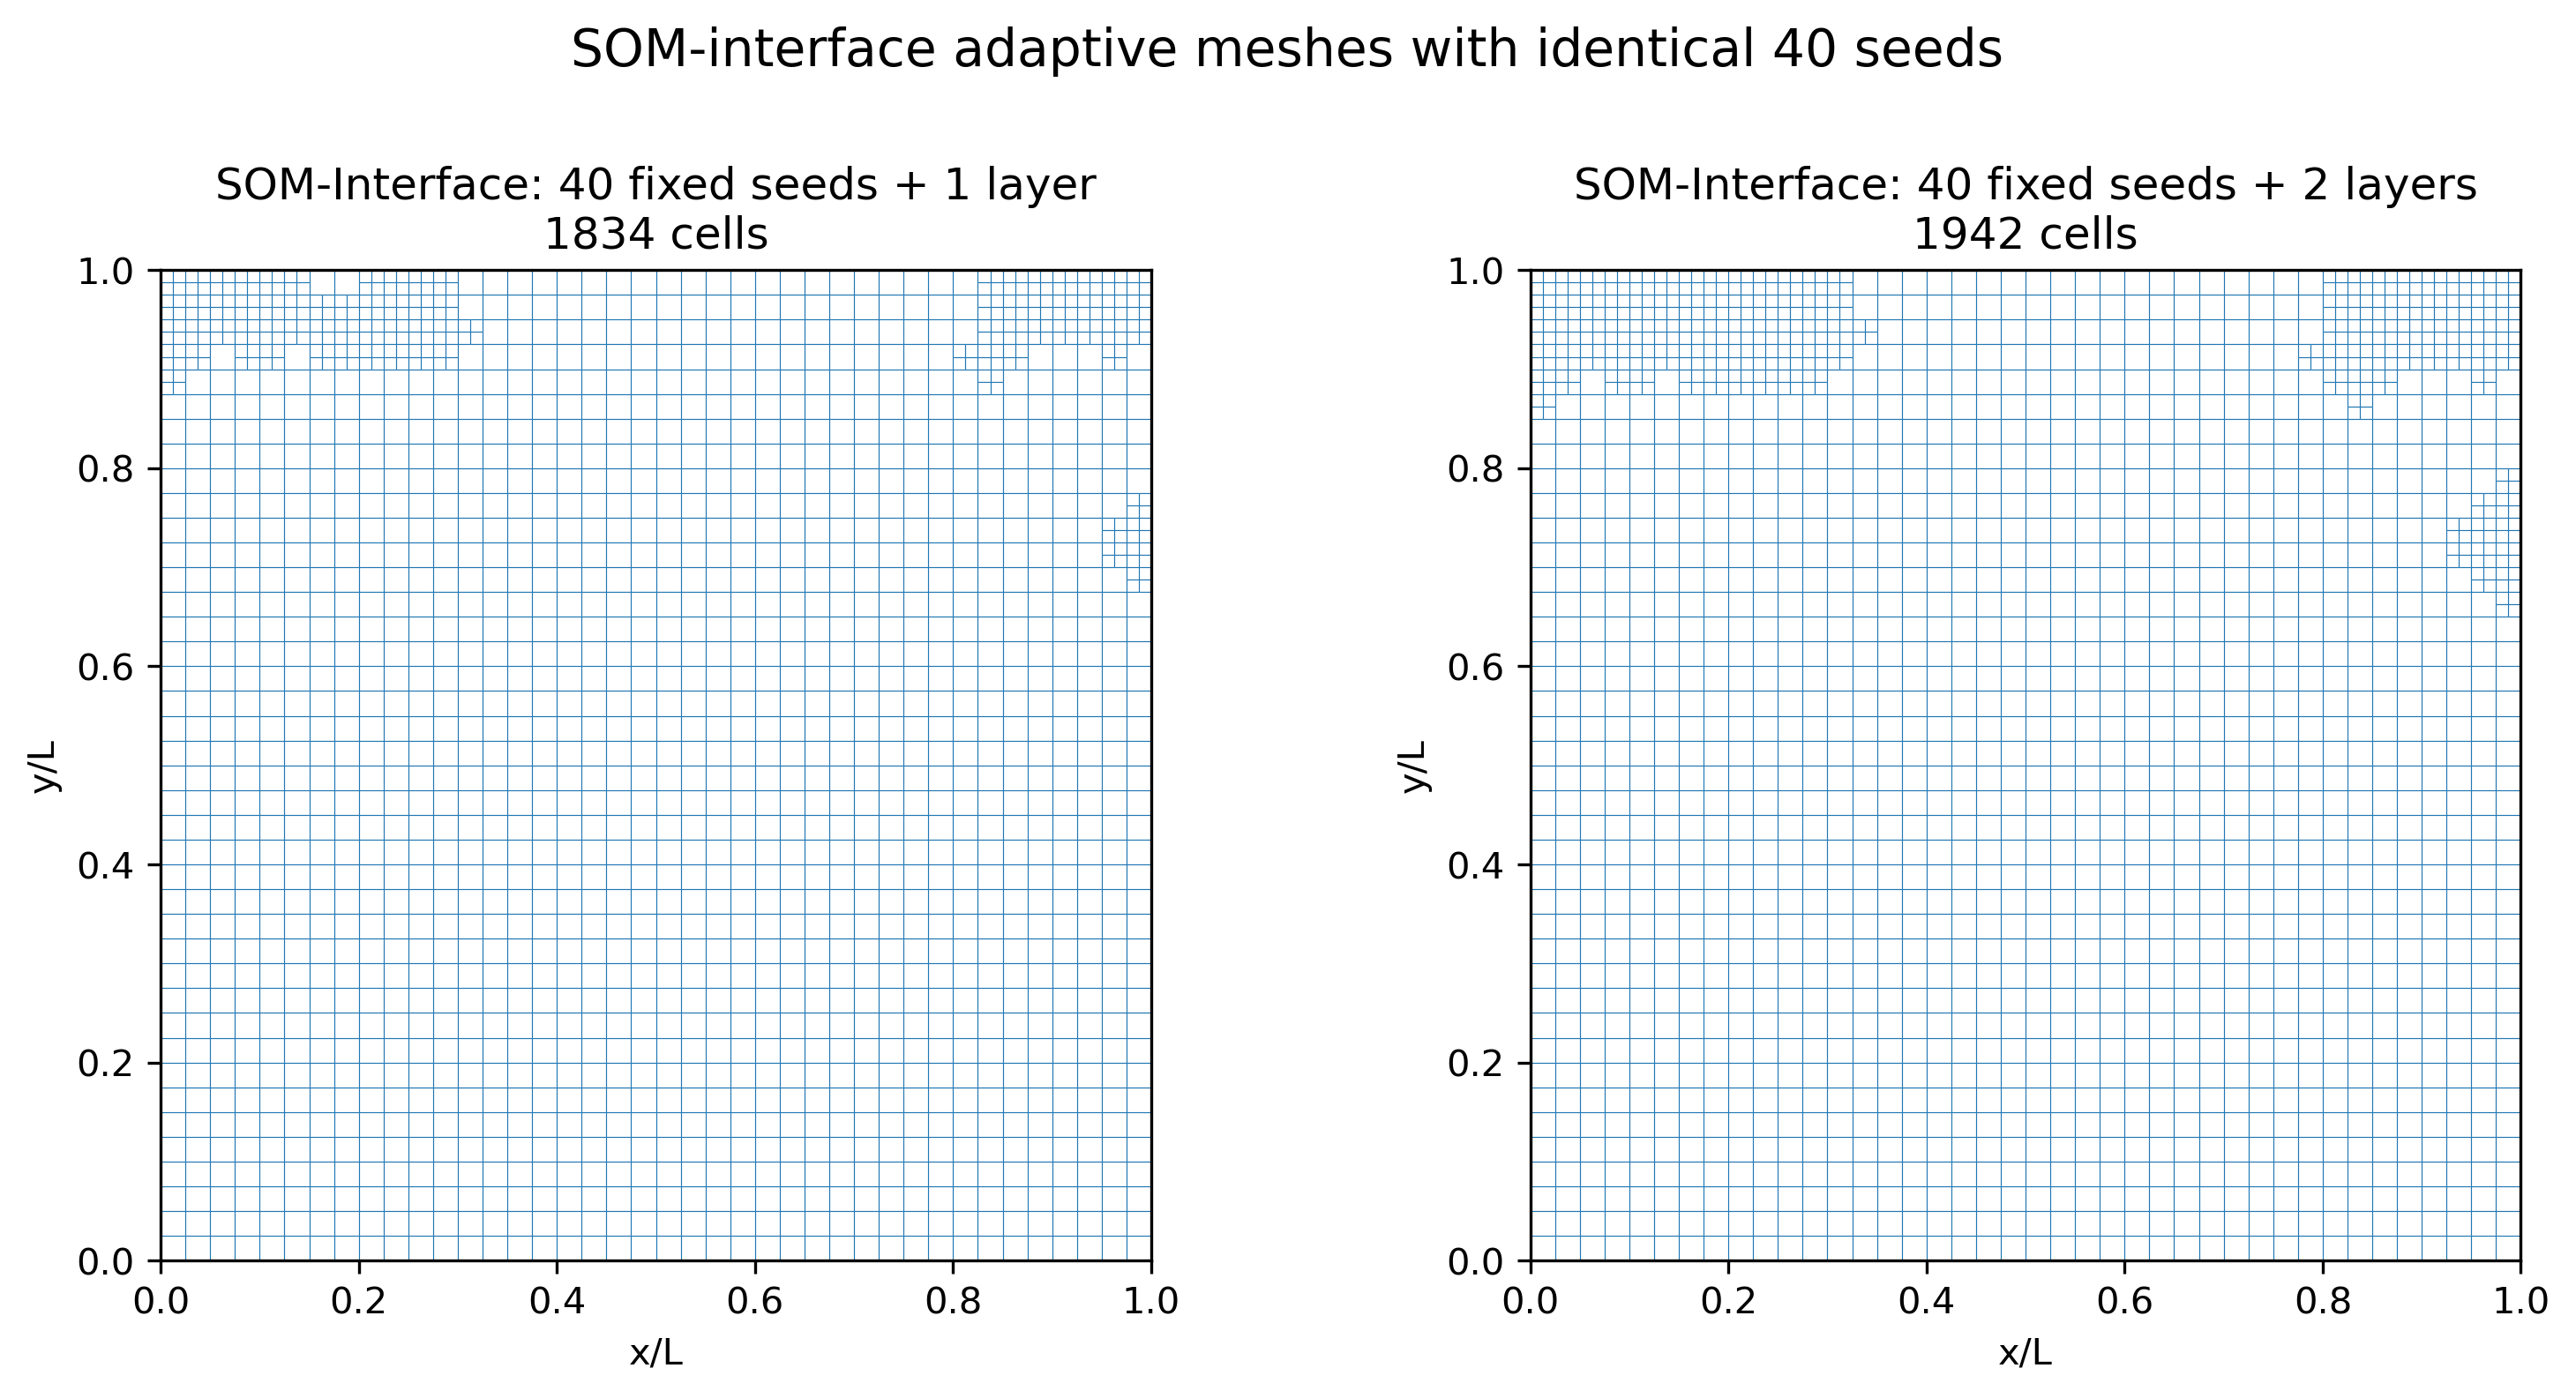
\includegraphics[width=0.92\textwidth]
{figures/SOM_Interface_real_mesh_1N_vs_2N.png}
\caption{Final adaptive meshes produced by the SOM-interface criterion using
the same 40 frozen interface seeds and one or two graph layers. The cases
contain 1834 and 1942 cells, respectively.}
\label{fig:som_interface_real_meshes}
\end{figure}

The real-mesh comparison shows that the second-stage criterion does not
simply refine isolated high-gradient cells. Instead, the fixed interface
seeds generate spatially connected refinement regions. Increasing the graph
radius from one to two layers preserves the same seed set and adds 36
additional cells, increasing the final mesh from 1834 to 1942 cells.

\begin{figure}[htbp]
\centering
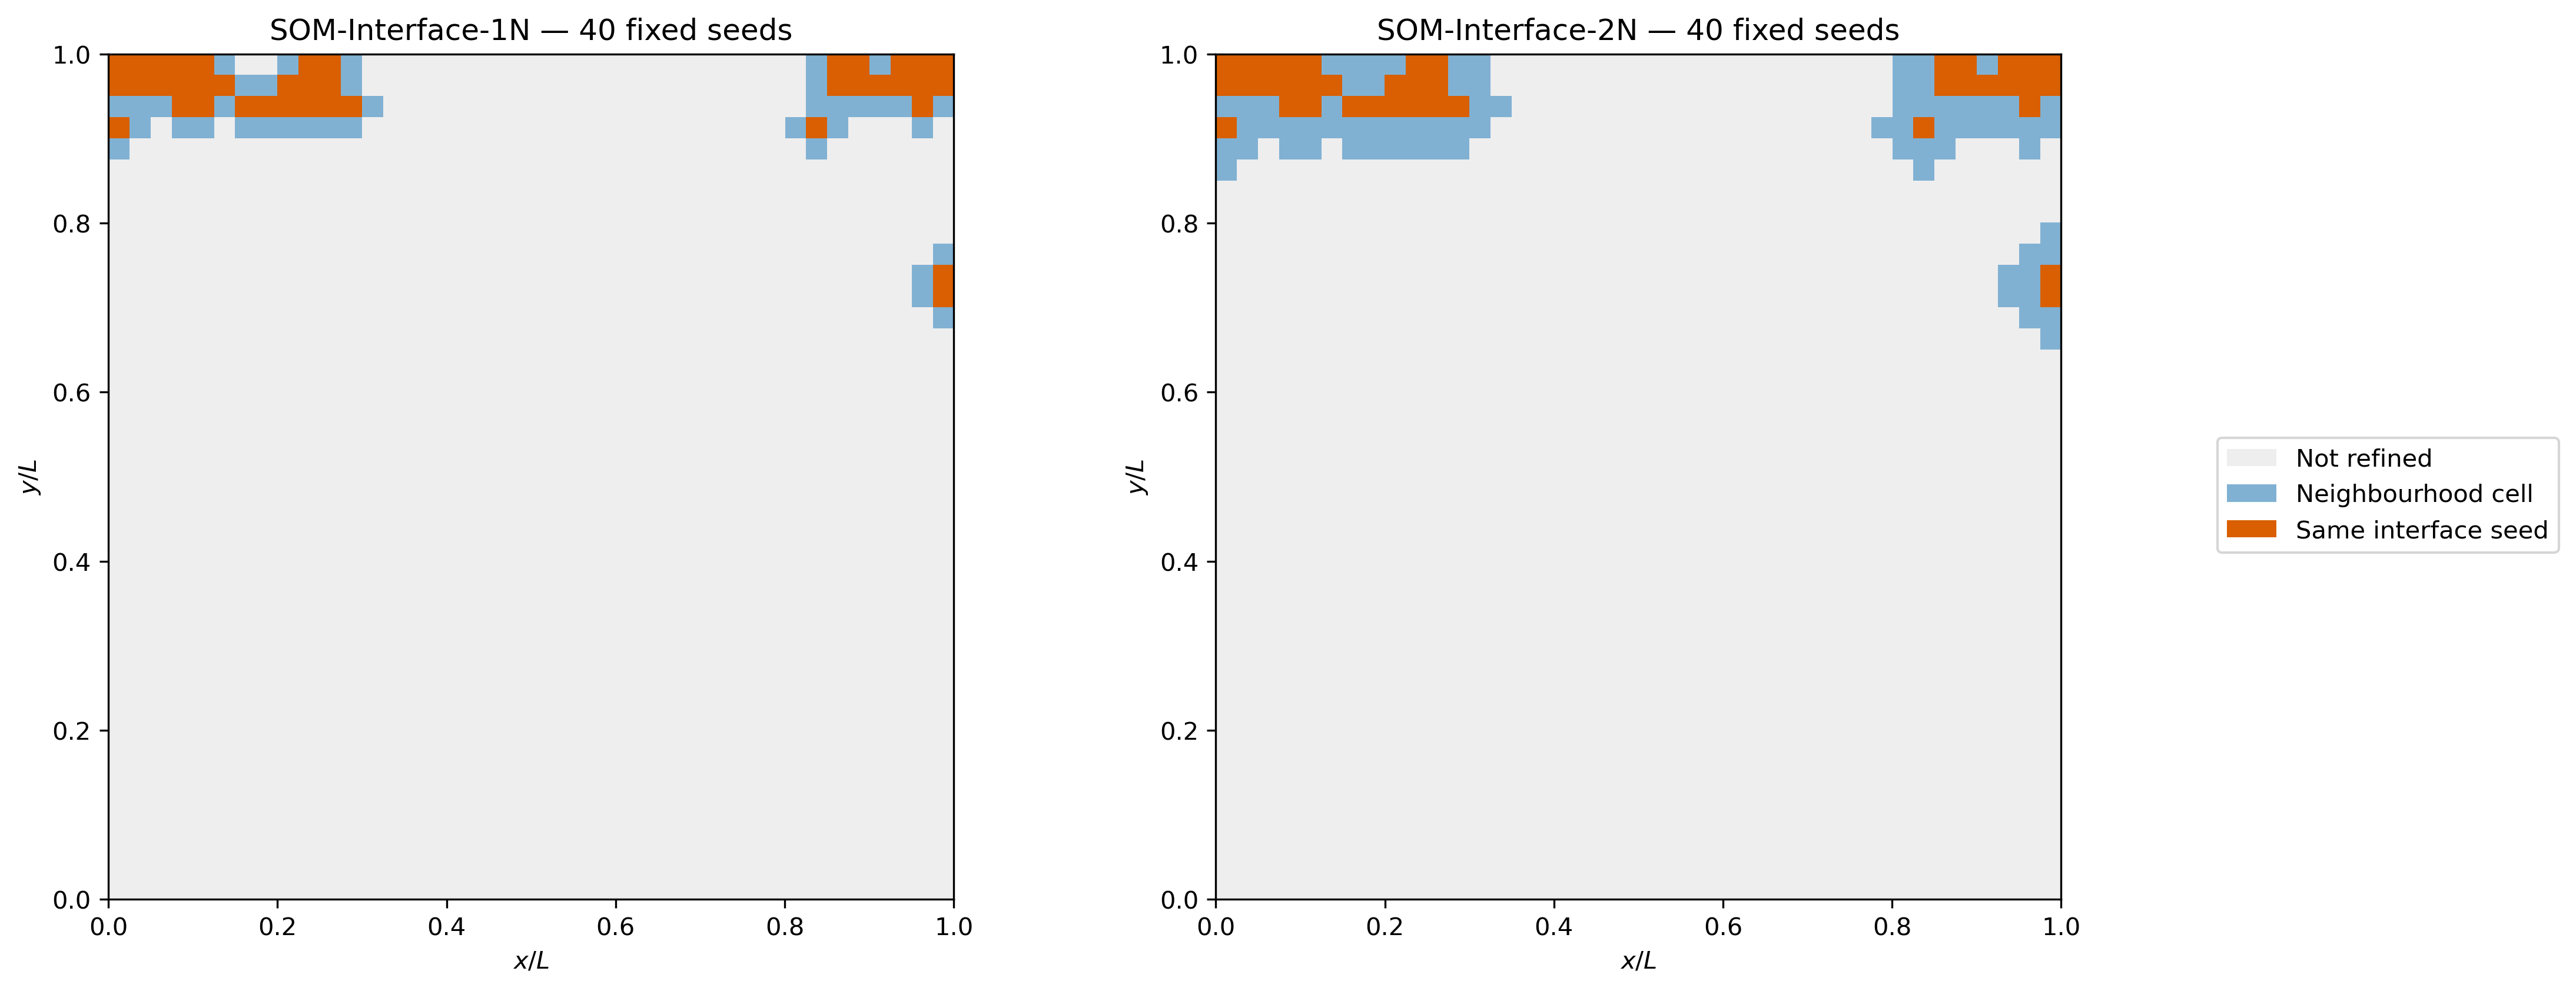
\includegraphics[width=0.88\textwidth]
{figures/SOM_Interface_fixed_seeds_1N_vs_2N.png}
\caption{Selection obtained from the same 40 frozen SOM-interface seeds for
one and two graph-layer expansions. The \(1N\) selection is a subset of the
\(2N\) selection; the latter adds 36 cells.}
\label{fig:som_interface_fixed_seeds}
\end{figure}

\subsection{Gradient versus SOM-interface selection overlap}

The cell-matched comparisons also show that the new criterion is related to,
but not identical with, the conventional Gradient criterion. For the
1834-cell comparison, 53 of the 78 selected cells were common to both
methods, corresponding to an overlap of \(67.95\%\). Each method selected
25 additional cells not selected by the other.

For the 1942-cell comparison, 74 of the 114 selected cells were common,
corresponding to an overlap of \(64.91\%\). Gradient selected 40 cells that
were not selected by SOM-interface, while SOM-interface selected another
40 cells.

\begin{figure}[htbp]
\centering
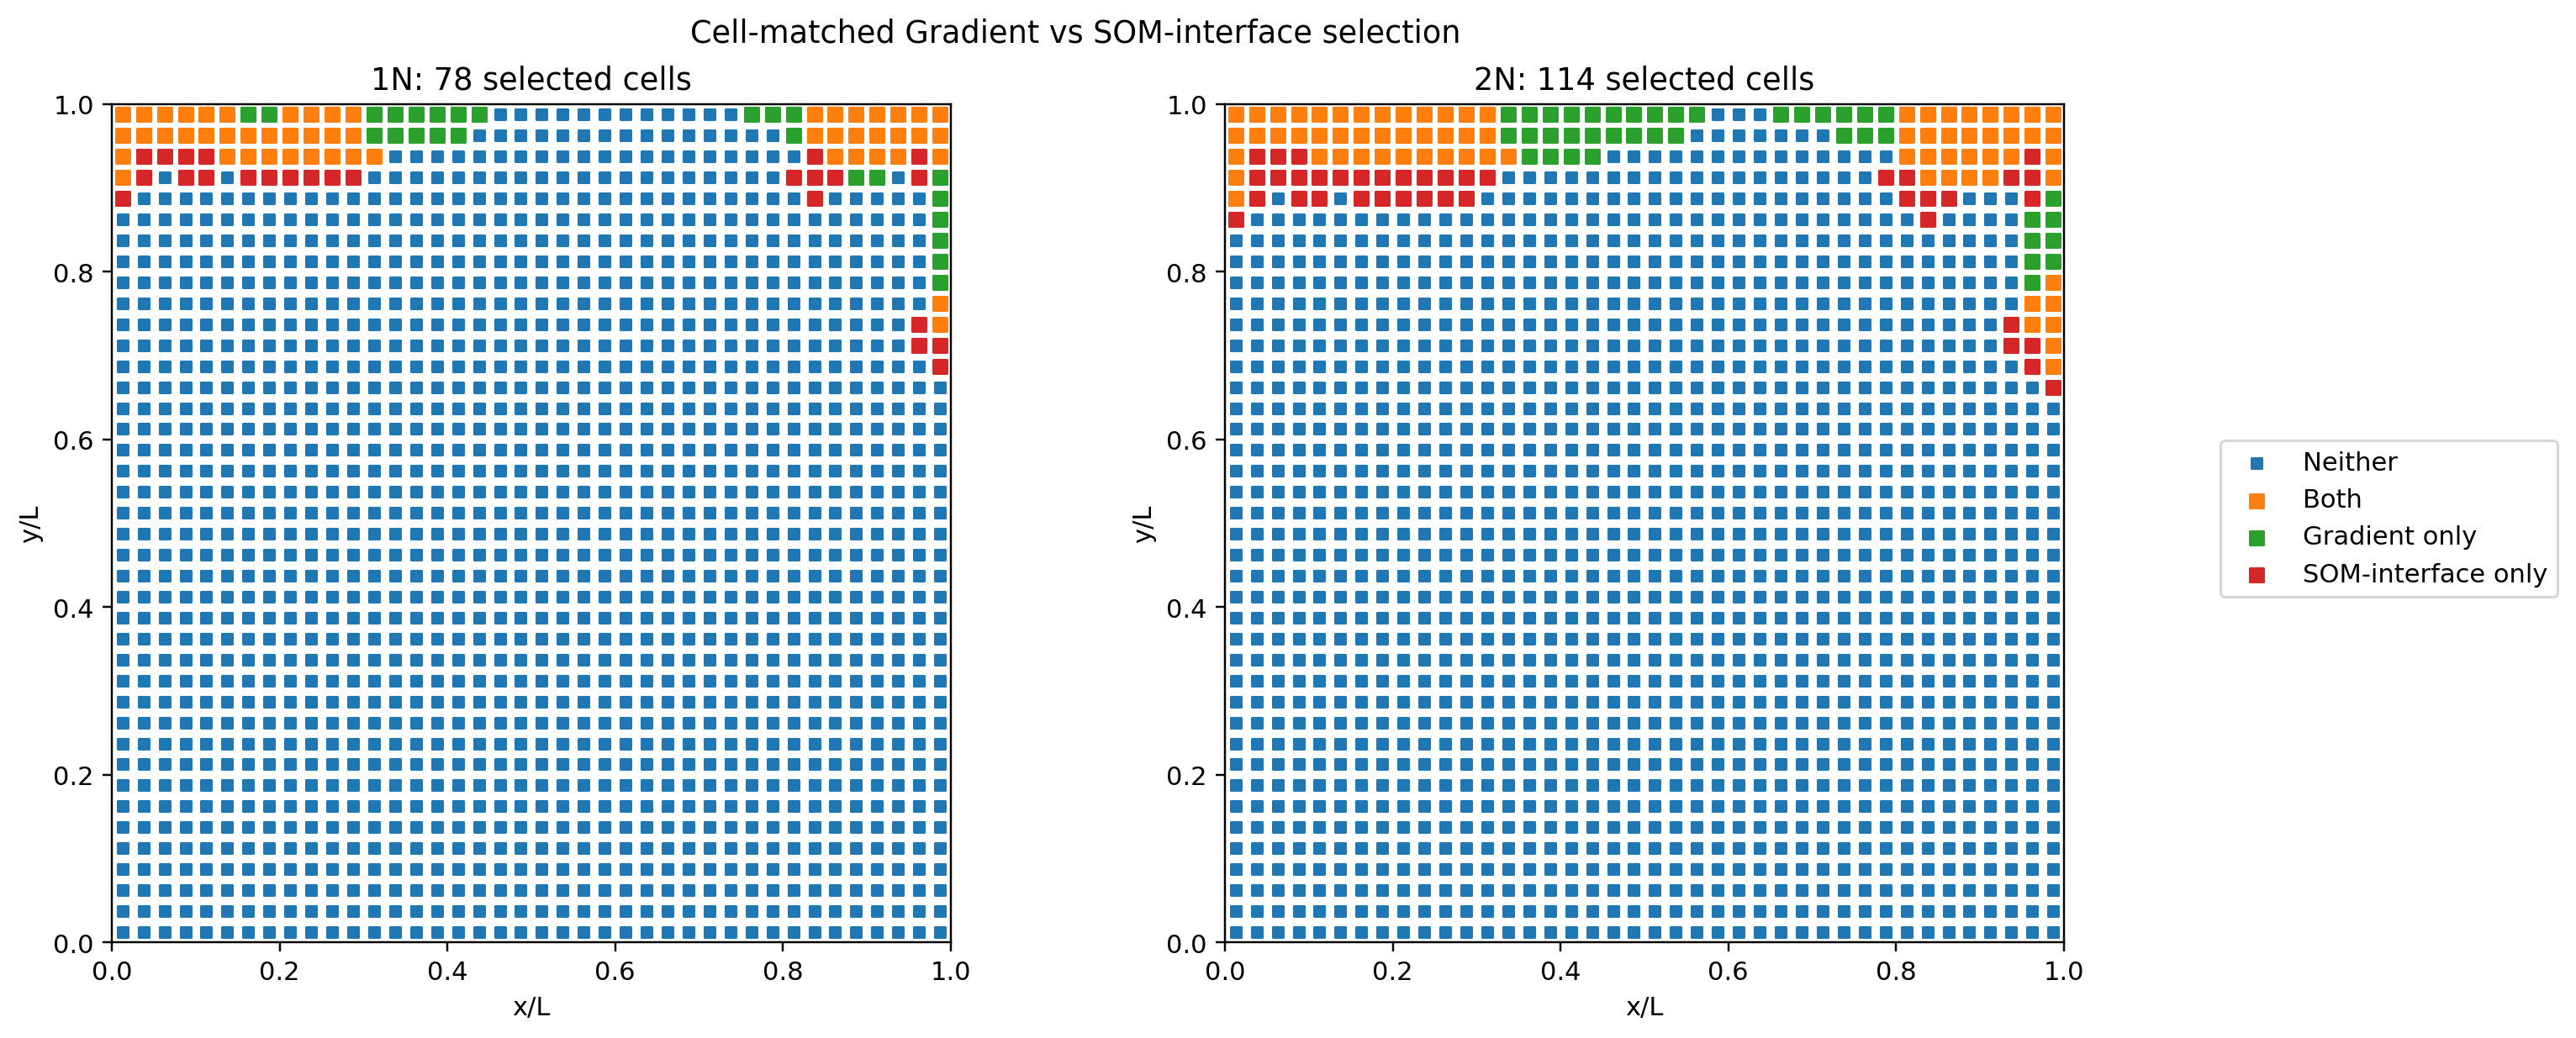
\includegraphics[width=0.90\textwidth]
{figures/Gradient_vs_SOM_Interface_cell_matched.png}
\caption{Cell-by-cell comparison between Gradient and SOM-interface
selections at matched final mesh sizes. The methods share a substantial
fraction of selected cells while allocating the remaining refinement budget
differently.}
\label{fig:gradient_som_interface_overlap}
\end{figure}

These overlaps are important because the new results cannot be explained by
a completely different refinement philosophy. A substantial portion of the
selected cells is common to both methods. The numerical differences arise
from the spatial allocation of the remaining refinement cells.

\subsection{SOM Architecture and Initialization Sensitivity}
\label{sec:som_sensitivity}

A sensitivity study was performed to determine how the SOM representation
depends on lattice architecture and random initialization. Four square
architectures were evaluated: \(3\times3\), \(4\times4\), \(5\times5\),
and \(6\times6\), corresponding to 9, 16, 25, and 36 neurons,
respectively.

For each architecture, five independent initializations were evaluated using
random seeds 1, 11, 21, 31, and 42, giving a total of 20 SOM training runs.
The M40 CFD solution, input features, feature standardization, SOM training
algorithm, and 20000 training iterations were held fixed across all runs.
The initial neighborhood width was also kept fixed at
\(\sigma_0=2\). Consequently, its size relative to the SOM lattice changes
with architecture; this choice was retained deliberately so that the tested
configurations differed only in lattice size and random initialization under
the common training specification.

The sensitivity analysis considered several complementary quantities:
quantization error, SOM-interface fraction, partition stability between
random initializations, and spatial stability of the 40 highest-priority
interface seeds. These metrics characterize different properties of the SOM
and should not individually be interpreted as measures of adaptive-mesh
accuracy.

Table~\ref{tab:som_architecture_sensitivity} summarizes the architecture-level
statistics obtained by averaging over the five random initializations.

\begin{table}[htbp]
\centering
\caption{Sensitivity of the SOM representation to lattice architecture.
Reported values are averages over five random seeds.}
\label{tab:som_architecture_sensitivity}
\begin{tabular}{cccccc}
\hline
Architecture & Neurons & Mean QE & SD QE & Interface fraction & Occupied neurons \\
\hline
\(3\times3\) & 9  & 0.6468 & 0.0136 & 0.3078 & 9.0 \\
\(4\times4\) & 16 & 0.5049 & 0.0166 & 0.4381 & 16.0 \\
\(5\times5\) & 25 & 0.4023 & 0.0036 & 0.5478 & 25.0 \\
\(6\times6\) & 36 & 0.3431 & 0.0037 & 0.6304 & 35.8 \\
\hline
\end{tabular}
\end{table}

Increasing the number of SOM neurons systematically reduced the mean
quantization error for the tested configurations. The mean QE decreased from
approximately 0.647 for the \(3\times3\) architecture to 0.343 for the
\(6\times6\) architecture. This behavior is expected because a larger number
of prototypes provides greater representational capacity in the standardized
feature space.

At the same time, the fraction of M40 cells classified as SOM-interface cells
increased substantially, from approximately 30.8\% for \(3\times3\) to
43.8\% for \(4\times4\), 54.8\% for \(5\times5\), and 63.0\% for
\(6\times6\). Thus, increasing SOM resolution produces a finer partition of
the CFD state space but also generates a progressively denser spatial
interface network.

The reduction in quantization error should therefore not be interpreted as
evidence that the larger SOM architectures are automatically preferable for
adaptive refinement. Quantization error measures representation in feature
space, whereas the usefulness of a SOM-derived refinement criterion depends
on how the resulting state partition and interfaces contribute to subsequent
mesh-refinement decisions.

\subsubsection{Partition stability across random initializations}

Because SOM training depends on initialization, the stability of the learned
cell partition was evaluated across the five random seeds. Direct comparison
of BMU labels is not sufficient because neuron labels can be permuted between
independent SOM trainings. Partition similarity was therefore evaluated using
the Adjusted Rand Index (ARI) and a same-cluster pairwise Jaccard measure.

\begin{table}[htbp]
\centering
\caption{Stability of the SOM partition across random initializations.
Statistics are calculated from pairwise comparisons between the five seeds
for each architecture.}
\label{tab:som_partition_stability}
\begin{tabular}{ccccc}
\hline
Architecture & Mean ARI & SD ARI & Mean pair Jaccard & SD pair Jaccard \\
\hline
\(3\times3\) & 0.901 & 0.021 & 0.847 & 0.029 \\
\(4\times4\) & 0.771 & 0.031 & 0.656 & 0.038 \\
\(5\times5\) & 0.795 & 0.043 & 0.679 & 0.058 \\
\(6\times6\) & 0.674 & 0.051 & 0.526 & 0.056 \\
\hline
\end{tabular}
\end{table}

The \(3\times3\) architecture produced the most stable partition among the
tested configurations, with a mean ARI of approximately 0.901. The
\(6\times6\) architecture produced the lowest mean ARI, approximately 0.674.
The behavior was not strictly monotonic with lattice size: the \(5\times5\)
architecture was somewhat more stable than the \(4\times4\) architecture
according to both partition metrics.

These results show that the reduction in quantization error obtained with
larger maps does not imply increased robustness to random initialization.
In particular, the \(6\times6\) configuration achieved the lowest mean
quantization error while also exhibiting the lowest partition stability of
the four architectures tested. Architecture selection therefore involves
more than minimizing quantization error alone.

\subsubsection{Spatial stability of high-priority interface seeds}

Partition stability does not by itself determine whether the cells considered
most important for refinement move to completely different physical regions.
The spatial stability of the 40 highest-priority SOM-interface seeds was
therefore evaluated separately.

\begin{table}[htbp]
\centering
\caption{Spatial stability of the 40 highest-priority SOM-interface seeds
across random initializations.}
\label{tab:som_spatial_stability}
\begin{tabular}{ccccc}
\hline
Architecture & Exact Jaccard & Exact match & \(r=1\) match & \(r=2\) match \\
\hline
\(3\times3\) & 0.698 & 0.820 & 0.955 & 0.986 \\
\(4\times4\) & 0.507 & 0.665 & 0.895 & 0.960 \\
\(5\times5\) & 0.551 & 0.708 & 0.931 & 0.970 \\
\(6\times6\) & 0.609 & 0.753 & 0.951 & 0.988 \\
\hline
\end{tabular}
\end{table}

Exact agreement between the Top-40 seed sets varied appreciably with random
initialization. For the \(4\times4\) architecture used in the main study,
the mean exact Jaccard similarity was approximately 0.507 and the mean exact
cell-match fraction was 0.665.

However, much of this variation was spatially local. When a selected cell
was considered matched if a corresponding selection occurred within one
M40 cell layer, the mean match fraction for the \(4\times4\) architecture
increased to approximately 0.895. With a two-cell-layer tolerance it
increased to approximately 0.960. Similar behavior was observed for the
other tested architectures.

These proximity statistics indicate that different initializations often
identify nearby regions even when they do not select exactly the same cells.
They should nevertheless be interpreted cautiously: the proximity measure
allows local many-to-one correspondence and is not equivalent to the overlap
of the final refined regions or to equality of the resulting adaptive CFD
solutions.

Figure~\ref{fig:som_sensitivity_consensus} provides a spatial view of these
sensitivity results. The upper row shows how frequently each M40 cell was
classified as a SOM-interface cell across the five random initializations,
whereas the lower row shows the corresponding selection frequency among the
40 highest-priority interface seeds.

\begin{figure}[htbp]
\centering
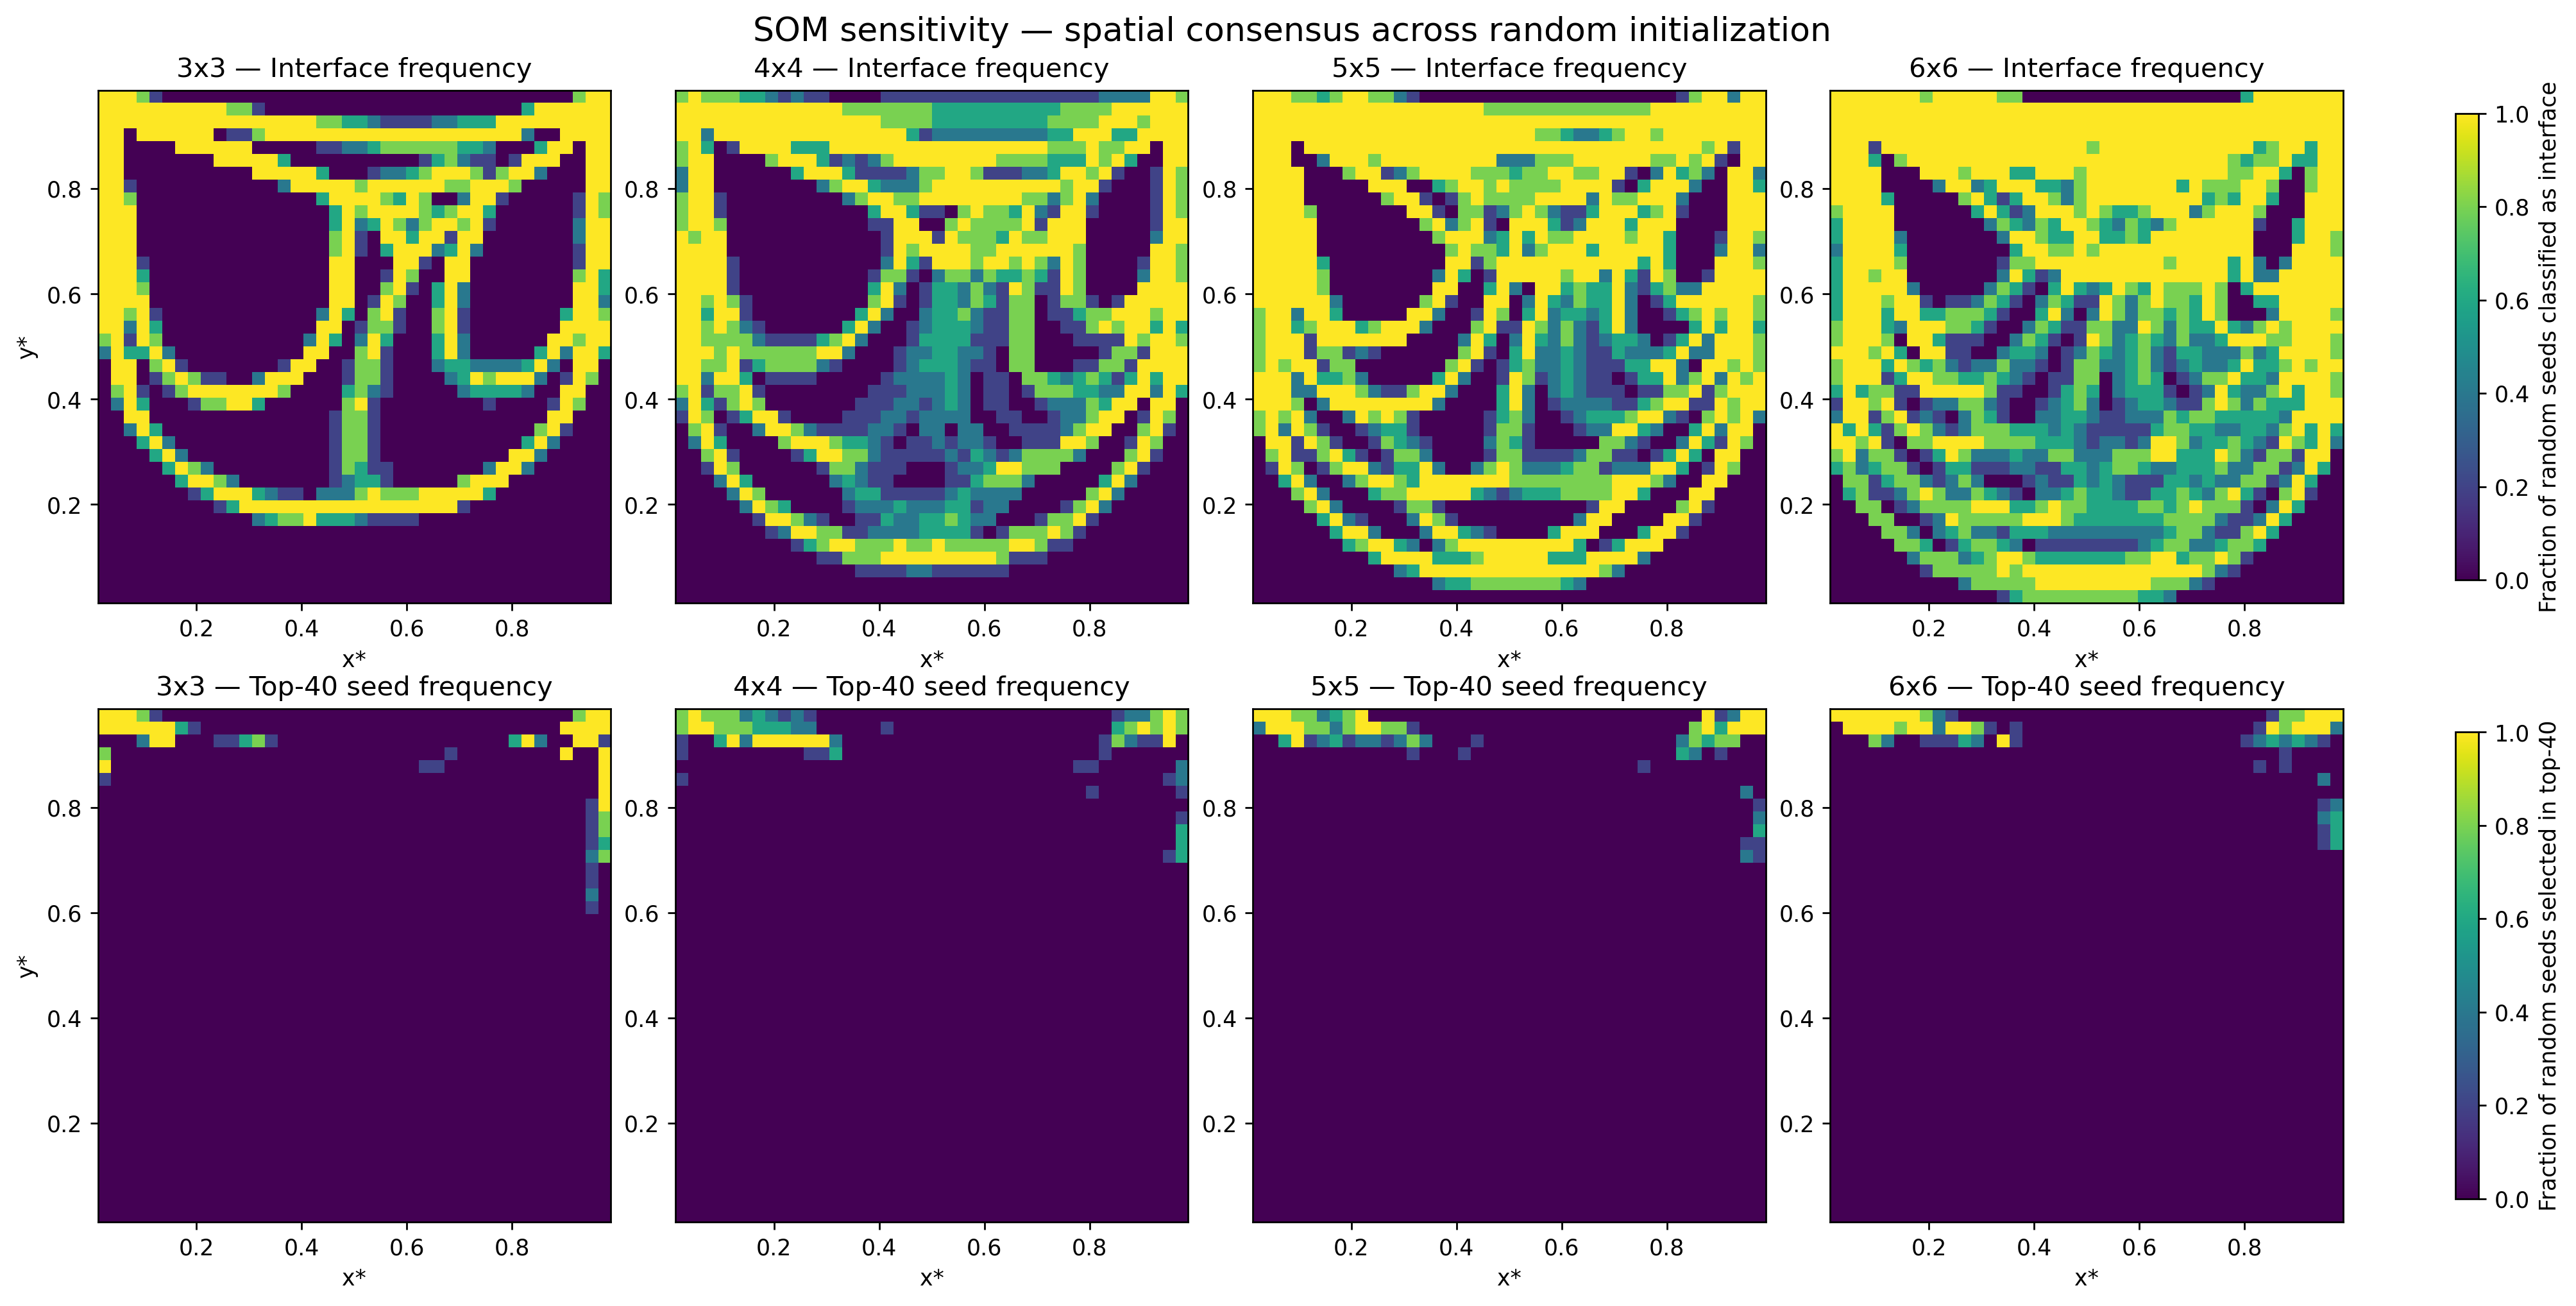
\includegraphics[width=0.98\textwidth]
{figures/som_sensitivity_consensus.png}
\caption{Spatial consensus across five random initializations for the
\(3\times3\), \(4\times4\), \(5\times5\), and \(6\times6\) SOM
architectures. The upper row shows SOM-interface frequency and the lower row
shows Top-40 seed-selection frequency.}
\label{fig:som_sensitivity_consensus}
\end{figure}

The consensus maps reinforce the quantitative results. Increasing the SOM
size produces a denser network of state interfaces, while the highest-priority
interface selections remain concentrated within comparatively localized
regions of the cavity. Differences between random initializations therefore
affect the exact partition and exact selected cells without necessarily
relocating all high-priority selections to unrelated physical regions.

The sensitivity study does not identify a uniquely optimal SOM architecture.
The \(3\times3\) map provides the highest partition stability but the
coarsest representation among the tested configurations. Conversely, the
\(6\times6\) map provides the lowest mean quantization error but generates
the densest interface network and exhibits the lowest mean partition
stability. The \(4\times4\) configuration used in the main adaptive study
should therefore be interpreted as the nominal architecture investigated in
that study, rather than as an architecture demonstrated to be optimal.

More generally, the results demonstrate that SOM architecture and random
initialization constitute relevant modeling choices for the proposed
interface-based refinement framework. Robustness of a fixed-seed result
should not be conflated with robustness to alternative initializations, and
future applications should evaluate architecture and initialization
sensitivity for the flow problem under consideration.


\subsection{Refinement-utility analysis}

To investigate whether the observed differences could be related to the
utility of the selected regions, the adaptive-mesh discrepancy fields were
interpolated back onto the original M40 cell centers. The M40--M160
discrepancy was used only as an evaluation quantity. Cells were partitioned
into four mutually exclusive groups: selected by both methods,
Gradient-only, SOM-only, and selected by neither method.

For the \(1N\) comparison, the mean M40 discrepancy in the common region was
\(2.91\times10^{-2}\). The corresponding post-refinement errors were
\(7.43\times10^{-3}\) for Gradient and \(1.05\times10^{-2}\) for
SOM-interface. In the Gradient-only region, the post-refinement errors were
\(3.60\times10^{-3}\) and \(6.31\times10^{-3}\), respectively. In the
SOM-only region they were \(4.55\times10^{-3}\) and \(4.91\times10^{-3}\).

For the \(2N\) comparison, the common region had a mean M40 discrepancy of
\(2.34\times10^{-2}\), with post-refinement errors of
\(6.44\times10^{-3}\) for Gradient and \(7.25\times10^{-3}\) for
SOM-interface. In the SOM-only region, however, SOM-interface produced a
lower mean post-refinement error than Gradient,
\(3.50\times10^{-3}\) versus \(3.84\times10^{-3}\).

The same analysis also shows that the benefit of either refinement strategy
is not confined to the cells explicitly selected for refinement. In the
regions selected by neither method, SOM-interface produced lower mean
post-refinement error than Gradient in both matched cases. This is
consistent with the globally coupled nature of the CFD solution and
reinforces the need to evaluate refinement strategies through the resulting
solution rather than through local indicator values alone.

\begin{table}[htbp]
\centering
\caption{Spatial refinement-utility analysis for the cell-matched
comparisons. ``SOM better fraction'' is the fraction of M40 locations in
each region for which the interpolated SOM-interface discrepancy is lower
than the corresponding Gradient discrepancy.}
\label{tab:refinement_utility_interface}
\small
\begin{tabular}{llrrrr}
\toprule
Case & Region & \(N\) & M40 error & Gradient error & SOM error \\
\midrule
1N & Both & 53 & 2.907e-2 & 7.434e-3 & 1.053e-2 \\
1N & Gradient-only & 25 & 1.058e-2 & 3.603e-3 & 6.306e-3 \\
1N & SOM-only & 25 & 1.032e-2 & 4.546e-3 & 4.910e-3 \\
1N & Neither & 1497 & 2.205e-3 & 1.523e-3 & 1.145e-3 \\
\midrule
2N & Both & 74 & 2.341e-2 & 6.445e-3 & 7.245e-3 \\
2N & Gradient-only & 40 & 5.936e-3 & 2.551e-3 & 2.940e-3 \\
2N & SOM-only & 40 & 9.194e-3 & 3.844e-3 & 3.496e-3 \\
2N & Neither & 1446 & 2.093e-3 & 1.332e-3 & 9.861e-4 \\
\bottomrule
\end{tabular}
\end{table}

The utility analysis should not be interpreted as a cell-level proof that
SOM-interface is universally superior. Rather, it provides evidence that
the new criterion changes the spatial distribution of refinement in a way
that can produce a different global solution response. In particular, the
\(2N\) case shows a lower error in the SOM-only region, while the common and
Gradient-only regions still favor Gradient on average.


\subsection{Final adaptive-mesh topology}

The differences between the refinement indicators can also be examined
directly through the final computational meshes. Figure~\ref{fig:adaptive_meshes}
compares the SOM-QE and Gradient meshes at the 10\% refinement budget.
Both simulations contain exactly 2080 cells and passed the OpenFOAM mesh
quality checks.

\begin{figure}[htbp]
\centering
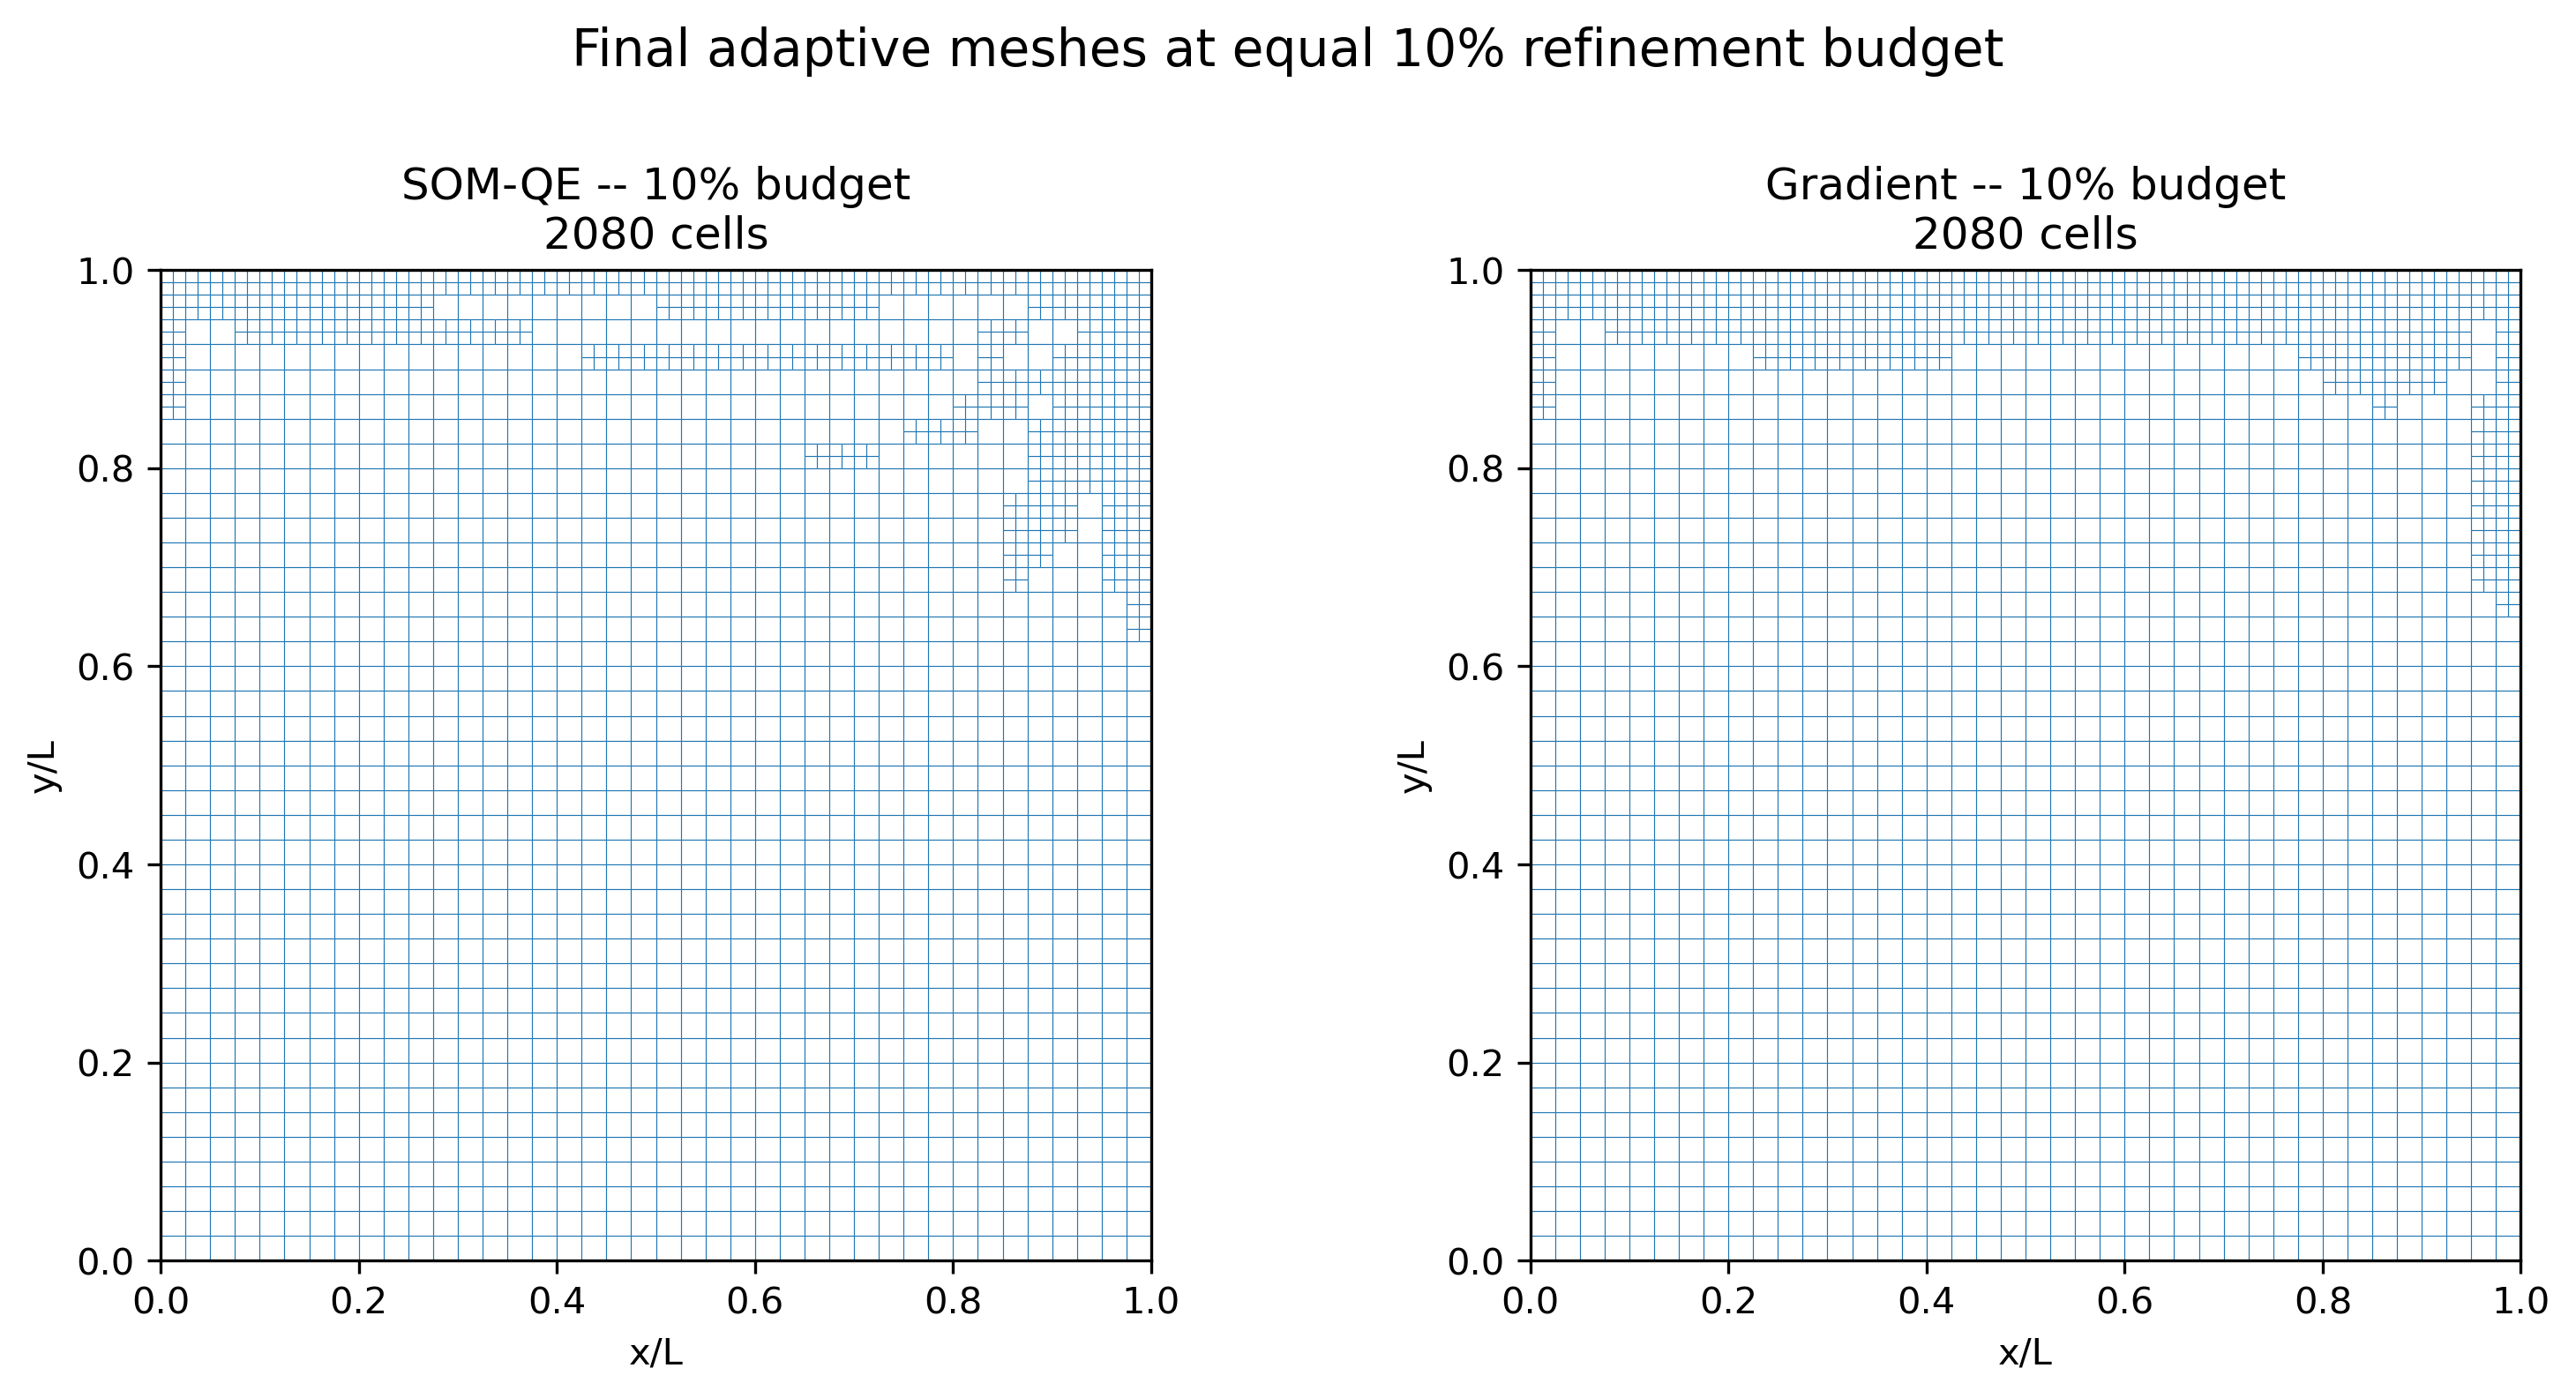
\includegraphics[width=0.98\textwidth]
{figures/Adaptive_mesh_SOM_vs_Gradient_10.png}
\caption{Final adaptive meshes obtained with SOM-QE and Gradient refinement
at the same 10\% refinement budget. Both meshes contain 2080 cells. The
comparison therefore isolates differences in the spatial allocation of
refinement rather than differences in total cell count.}
\label{fig:adaptive_meshes}
\end{figure}

The two indicators allocate the identical refinement budget differently.
Gradient concentrates refinement predominantly near the moving lid and the
upper cavity, where large velocity gradients occur. SOM-QE also refines the
upper region but distributes part of its refinement budget into additional
flow regions extending farther into the cavity.

This distinction is important because the adaptive-mesh comparison shows
that equal numbers of cells do not imply equal numerical performance.
At the 10\% budget, the Gradient mesh produces a lower RMS discrepancy
relative to the M160 reference despite having exactly the same number of
cells as the SOM-QE mesh. The result therefore points to the spatial
allocation of refinement, rather than cell count alone, as the relevant
difference between the two strategies.



\section{Discussion}
\label{sec:discussion}

\subsection{Why direct SOM-QE refinement did not outperform Gradient}

The controlled adaptive-mesh experiments provide a clear result for the
present lid-driven-cavity problem: direct refinement based on SOM
quantization error does not outperform the conventional velocity-gradient
indicator.

This result is particularly relevant because the preliminary indicator
analysis initially suggested that SOM-QE contained potentially useful
information. On the M40 pilot solution, quantization error was spatially
correlated with regions exhibiting relatively large discrepancies with the
M160 reference. At some refinement budgets, ranking cells by SOM-QE captured
a substantial fraction of the initial M40--M160 discrepancy.

However, the adaptive simulations demonstrate that identifying cells with
large current discrepancy is not equivalent to identifying cells whose
refinement will produce the largest reduction in the final global error.

The distinction may be written conceptually as

\begin{equation}
\text{current local discrepancy}
\neq
\text{refinement utility}.
\end{equation}

Refinement modifies the discrete CFD system itself. The resulting velocity
field is globally coupled through the governing equations, pressure--velocity
interaction, boundary conditions, and neighboring control volumes.
Consequently, refining one region can improve the solution in locations that
were not directly selected for refinement.

This behavior was observed explicitly in the 10\% refinement-benefit
analysis. Gradient refinement improved the solution over a broad fraction of
the common diagnostic grid, including regions not directly selected by the
Gradient criterion. SOM-QE refinement produced a smaller global benefit and
even increased the local discrepancy in portions of the unselected domain.

Therefore, the value of a refinement indicator cannot be established solely
from its correlation with an existing error field. It must ultimately be
evaluated through the solution obtained after refinement.

\subsection{What the SOM actually learned}

The inferior performance of direct SOM-QE refinement should not be
interpreted as evidence that the SOM failed to learn meaningful information
about the flow.

The SOM was trained using local flow variables and velocity-gradient
information without including the spatial coordinates \(x/L\) and \(y/L\)
as input features. Nevertheless, the resulting best-matching-unit
classification formed spatially coherent regions when mapped back onto the
cavity.

This indicates that the SOM identified recurring local flow states rather
than merely memorizing spatial position.

Analysis of the SOM neurons further showed that cells having comparable
velocity-gradient magnitudes could belong to different neurons because their
velocity magnitude and directional components differed. In this sense, the
Gradient indicator and the SOM encode different types of information:

\begin{equation}
\text{Gradient}
\rightarrow
\text{strength of local solution variation},
\end{equation}

whereas

\begin{equation}
\text{SOM state}
\rightarrow
\text{type of local flow regime}.
\end{equation}

This distinction explains why SOM-based information can be physically
structured without automatically becoming an effective numerical-error
indicator.

\subsection{Quantization error is not an error estimator}

SOM quantization error measures the distance between an input sample and its
best-matching SOM prototype in standardized feature space. A large value
therefore indicates that the local flow state is represented relatively
poorly by the trained map.

It does not, by definition, measure discretization error.

In the present case, SOM-QE and velocity-gradient magnitude were strongly
correlated. Their cell-level correlation was approximately

\begin{equation}
r\left(|\nabla U|,QE\right)=0.879.
\end{equation}

Both quantities therefore respond strongly to extreme flow states, including
the upper-corner regions associated with the moving-lid boundary condition.

This explains why SOM-QE initially appeared promising as an error-location
indicator. Nevertheless, the adaptive experiments separate correlation from
causation: the cells with the largest quantization error are not necessarily
the cells whose refinement most efficiently reduces the global CFD
discrepancy.

For the present experiment, the hypothesis that SOM quantization error can
serve directly as a superior refinement indicator is therefore not
supported.

\subsection{Interpretation of the final adaptive meshes}

The final 10\% adaptive meshes provide a geometric interpretation of the
quantitative results.

Both SOM-QE and Gradient begin from the same M40 pilot mesh, select the same
number of cells for refinement, and produce final meshes containing 2080
cells. Nevertheless, Figure~\ref{fig:adaptive_meshes} shows that the cells
are distributed differently.

The Gradient criterion concentrates a larger fraction of the available
resolution close to the moving lid and upper cavity, where the velocity
field changes rapidly. SOM-QE allocates part of the same finite refinement
budget to additional regions farther from the lid.

Those additional SOM-selected regions are not random. They correspond to
flow states that the SOM regards as unusual or poorly represented.
The adaptive CFD results nevertheless show that resolving those states more
finely does not produce as much global numerical benefit as concentrating
the same computational resources according to the Gradient criterion.

This provides an important engineering distinction:

\begin{equation}
\text{physically interesting}
\neq
\text{numerically profitable to refine}.
\end{equation}

For adaptive CFD, the objective is not merely to identify interesting flow
structures, but to allocate a limited computational budget where additional
resolution most improves the quantities of interest.

\subsection{What was learned from Hybrid-v1}

The Hybrid-v1 indicator was deliberately designed after rejecting direct
SOM-QE refinement as the primary strategy. Instead of allowing SOM
information to replace the conventional indicator, the velocity gradient
remained dominant and the SOM regime-transition indicator only modified its
priority:

\begin{equation}
I_{\mathrm{hyb},i}
=
G_i^{*}
\left(
1+\alpha T_i
\right),
\qquad
\alpha=0.5.
\end{equation}

The coefficient was fixed before evaluating the hybrid cases against the
M160 reference. It was not optimized using the reference solution.

This formulation produced a controlled perturbation of the Gradient
selection. Depending on refinement budget, approximately 91--96\% of the
Gradient-selected cells were retained.

The cells introduced by Hybrid-v1 consistently had somewhat smaller velocity
gradients but substantially larger SOM regime-transition indicators than the
cells they replaced. The algorithm therefore behaved according to its
intended design.

At the 10\% budget, changing only 11 of the 160 Gradient-selected cells
produced an approximately 1.24\% reduction in RMS discrepancy. However, the
same mechanism did not improve RMS performance at the 5\%, 15\%, or 20\%
budgets.

The appropriate conclusion is therefore not that the hybrid method improves
Gradient refinement. Rather, the experiment demonstrates that SOM-derived
flow-state information can alter refinement decisions in a controlled and
physically interpretable way, while the numerical value of those changes
remains dependent on the specific cells exchanged.

\subsection{Refinement utility as the central problem}

The combined results suggest a more precise research question for future
work.

The original question can be formulated as whether a SOM can identify cells
that should be refined. The present results indicate that this formulation
is too broad. A more useful question is:

\begin{quote}
What information learned by a SOM, if any, is predictive of the numerical
utility of refining a cell or region?
\end{quote}

This distinction changes the role of machine learning in the adaptive
workflow.

Rather than asking an unsupervised model to replace established numerical
indicators, a more defensible strategy is to use conventional physics-based
or numerical indicators as the primary refinement signal and investigate
whether learned flow-state information can improve decisions near the
refinement threshold.

The Hybrid-v1 experiment represents a first controlled test of this concept,
but the present evidence is insufficient to establish a general advantage.


\subsection{Reframing the SOM evaluation}

The direct SOM-QE results changed the research question rather than ending
the investigation. Quantization error was shown not to be a reliable direct
proxy for discretization error or refinement utility. The subsequent
analysis therefore used the SOM in a different role: identifying interfaces
between distinct learned flow states.

This distinction is important. A SOM does not need to predict numerical
error directly for its representation of the flow to be useful. It may
instead identify spatial structures that complement a conventional
numerical indicator. The SOM-interface criterion was constructed around
this hypothesis.

The new indicator combines three pieces of information available from the
M40 pilot solution:

\begin{equation}
I_{\mathrm{SI}}
=
T\sqrt{G^*\Delta U^*}.
\end{equation}

The transition term identifies a change in learned flow regime, while the
gradient and velocity-jump terms retain sensitivity to the local strength of
the physical variation. The resulting refinement is therefore not a pure
machine-learning replacement of Gradient. It is a physics-informed use of
the SOM representation.

\subsection{Cell-matched evaluation of SOM-interface}

A direct comparison at a nominal 10\% budget would have been misleading for
the new criterion because fixed-seed graph expansion naturally produces a
different number of selected cells. The experiments were therefore followed
by cell-matched Gradient controls.

The \(1N\) SOM-interface case selected 78 cells and was compared with a
Gradient selection of exactly 78 cells. The \(2N\) case selected 114 cells
and was compared with exactly 114 Gradient-selected cells. In both cases,
the final meshes therefore contained identical numbers of cells.

Under this controlled comparison, SOM-interface produced lower
volume-weighted mean and RMS discrepancies than the corresponding Gradient
case. The mean discrepancy reduction was approximately \(13.9\%\) for the
\(1N\) comparison and \(18.7\%\) for the \(2N\) comparison. The RMS reduction
was smaller, approximately \(1.4\%\) and \(4.0\%\), respectively.

The result is noteworthy because the methods shared a substantial fraction
of their selected cells, yet allocated the remaining cells differently.
The overlap decreased from \(67.95\%\) in the \(1N\) comparison to \(64.91\%\)
in the \(2N\) comparison.

The observed improvement should nevertheless be interpreted carefully. The
maximum pointwise discrepancy remained essentially unchanged between the
paired cases, and the simulations represent only one Reynolds number and
one cavity geometry. The present evidence therefore supports the statement
that the SOM-interface hypothesis is promising for this controlled test,
not that the method has been established as a generally superior adaptive
strategy.

\subsection{Why the new result is different from SOM-QE}

The contrast between SOM-QE and SOM-interface is itself an important result.
SOM-QE ranks cells according to how poorly their local feature vector is
represented by a SOM prototype. SOM-interface instead uses the spatial
organization of the BMU classification.

Consequently,

\begin{equation}
QE
\rightarrow
\text{representation mismatch},
\end{equation}

whereas

\begin{equation}
T
\rightarrow
\text{learned flow-state transition}.
\end{equation}

The second-stage criterion further combines the transition with local
physical variation. The new result therefore does not contradict the
earlier negative SOM-QE experiment. It tests a different hypothesis about
what information in the SOM may be useful for mesh adaptation.

\subsection{Interpretation of the refinement-utility analysis}

The cell-matched utility analysis provides a more nuanced interpretation
than simply comparing global mean and RMS values. In the common selected
region, Gradient produced lower mean post-refinement error in both the
\(1N\) and \(2N\) comparisons. Gradient also produced lower mean error in the
Gradient-only region.

In contrast, the SOM-interface selection showed lower mean error in the
SOM-only region for the \(2N\) case, and the SOM-interface solution also
showed lower mean error in the large region selected by neither method.
These observations indicate that the global improvement cannot be reduced
to a statement that every SOM-selected cell is individually more useful
than every Gradient-selected cell.

The result is consistent with the global coupling of the CFD equations.
Refinement changes the solution throughout the computational domain, so
the numerical value of a refinement decision must ultimately be evaluated
through its downstream effect on the complete solution.

The utility analysis therefore supports a more cautious interpretation:
the SOM-interface criterion appears to identify a different set of spatial
structures whose refinement can alter the global solution beneficially,
but the causal relationship between individual selected cells and global
error reduction remains unresolved.


\subsection{Engineering implications}

The study illustrates a broader methodological point for machine-learning
applications in computational engineering.

A machine-learning indicator can exhibit spatial structure, correlate with a
reference discrepancy, and identify physically meaningful flow regimes while
still failing to improve the final numerical solution.

For this reason, evaluation should proceed through a hierarchy of evidence:

\begin{enumerate}
    \item verify the underlying CFD solution;
    \item determine what information the machine-learning model actually
    represents;
    \item compare the proposed indicator against a conventional baseline at
    equal computational budgets;
    \item solve the adapted CFD cases rather than evaluating indicator
    correlation alone;
    \item assess the final quantities of interest and global error metrics;
    \item account for the complete computational cost before making
    efficiency claims.
\end{enumerate}

Within the original four-budget SOM-QE/Hybrid-v1 matrix, the conventional
Gradient indicator remains the most consistently accurate baseline. The
subsequent SOM-interface experiments provide a different and more promising
result in cell-matched tests, but they are not yet sufficient to establish
general superiority. The principal contribution of the combined analysis is
therefore the development and testing of a more precise hypothesis: learned
flow-regime information may be useful for adaptive refinement when it is
combined with physically meaningful measures of local variation and
evaluated through the resulting CFD solution.



\section{Limitations}
\label{sec:limitations}

The present study is intended as a controlled computational investigation
rather than as a demonstration of a generally applicable adaptive-meshing
method. Several limitations must therefore be considered when interpreting
the results.

\subsection{Fine-grid numerical reference}

The M160 solution is used throughout the adaptive-mesh analysis as a
fine-grid numerical reference. It should not be interpreted as an exact
solution.

Consequently, quantities reported as errors relative to M160 are more
precisely numerical discrepancies with respect to the finest solution used
in this study. Although the uniform-mesh sequence showed strong convergence
toward M160, a remaining discretization error is necessarily present in the
reference itself.

The results therefore support comparisons between refinement strategies
under a common reference, but they do not establish absolute discretization
errors.

\subsection{Spatial and temporal discretization}

The uniform-grid convergence study changed the time step together with the
spatial resolution. The reported M20--M40, M40--M80, and M80--M160
differences therefore do not isolate spatial discretization error
independently from temporal discretization effects.

The observed convergence rates are consistent with strong numerical
convergence of the tested sequence, particularly on the finer meshes, but
they should not be interpreted as a rigorous spatial order-of-accuracy
verification.

A future verification study should independently refine the time step and
the spatial mesh.

\subsection{Lid-driven-cavity corner behavior}

The moving lid meets stationary side walls at the upper corners of the
cavity. This discontinuity in the imposed wall velocity generates strong
local gradients and influences pointwise discrepancy measures.

The largest M40--M160 velocity discrepancy occurs close to the upper-right
corner, and a substantial fraction of the squared discrepancy is
concentrated in a relatively small number of cells near the upper boundary.

This behavior can influence both conventional gradient indicators and
SOM-derived quantities. In particular, the observed correlation between
quantization error and the M40--M160 discrepancy is partly associated with
both quantities responding strongly to extreme upper-corner flow states.

For this reason, maximum pointwise discrepancy is not used as the primary
criterion for comparing adaptive strategies. Volume-weighted mean and RMS
metrics provide more representative global measures for the present study.

\subsection{Single flow configuration}

All adaptive experiments were performed for the two-dimensional
lid-driven-cavity problem at

\begin{equation}
Re=100.
\end{equation}

The conclusions therefore apply only to the tested configuration.

No evidence is presently available to determine whether the relative
behavior of Gradient, SOM-QE, and Hybrid-v1 persists at different Reynolds
numbers, for different geometries, in three-dimensional flows, or for
problems involving heat transfer, turbulence, compressibility, multiphase
phenomena, or other physical processes.

Generalization must therefore be tested rather than assumed.

\subsection{SOM architecture and feature selection}

The adaptive CFD experiments in this investigation use a nominal
\(4\times4\) SOM containing 16 neurons and trained using the selected
velocity and velocity-gradient features. A separate sensitivity study
evaluated \(3\times3\), \(4\times4\), \(5\times5\), and \(6\times6\)
architectures across five random initializations. That analysis quantified
changes in representation error, partition stability, interface density,
and spatial stability of the high-priority interface seeds.

The sensitivity study does not establish an optimal SOM architecture and
does not repeat the complete adaptive CFD calculation for every architecture
and initialization. Consequently, it characterizes robustness of the learned
SOM partition and refinement-selection structure, rather than robustness of
the final adaptive CFD accuracy across all tested SOM configurations.

Similarly, the failure of direct SOM-QE refinement should not be interpreted
as a general failure of self-organizing maps for adaptive CFD. It establishes
only that quantization error from the present SOM configuration did not
provide a superior direct refinement criterion for the tested problem.

Alternative features, SOM dimensions, training procedures, or derived
indicators may produce different behavior. Such alternatives should,
however, be defined without tuning against the numerical reference used for
final evaluation.

\subsection{Hybrid-v1 is not optimized}

Hybrid-v1 uses

\begin{equation}
I_{\mathrm{hyb}}
=
G^{*}(1+0.5T).
\end{equation}

The coefficient \(\alpha=0.5\) was intentionally fixed rather than optimized
against M160. This prevents the reference solution from being used both to
design and evaluate the indicator.

Consequently, Hybrid-v1 should be interpreted as a proof-of-concept test of
whether SOM regime-transition information can modify a conventional
indicator in a controlled manner. It is not presented as an optimized
adaptive-meshing algorithm.

The isolated improvement observed at the 10\% budget is insufficient to
establish superiority over Gradient.

\subsection{Refinement-budget range}

Only four refinement budgets were investigated:

\begin{equation}
5\%,\qquad10\%,\qquad15\%,\qquad20\%.
\end{equation}

These experiments are sufficient to reveal important differences in
monotonicity and relative behavior, but they do not fully characterize the
accuracy--cost response of each method.

In particular, the present results should not be extrapolated to very small
or very large refinement fractions without additional simulations.

\subsection{Computational-cost measurements}

The reported execution times correspond to individual CFD solves and were
obtained from single runs. They are therefore susceptible to normal
variability in workstation load and operating-system scheduling.

Furthermore, the timings do not include the complete adaptive workflow,
which may contain:

\begin{itemize}
    \item the pilot CFD calculation;
    \item feature extraction;
    \item SOM training;
    \item indicator calculation;
    \item cell selection;
    \item mesh refinement;
    \item field transfer and post-processing.
\end{itemize}

No claim of computational-speed superiority is therefore made.

A rigorous efficiency study should use repeated timing measurements and
compare total workflow cost for a specified accuracy or quantity-of-interest
target.

\subsection{Refinement strategy}

The current framework performs one refinement operation based on information
from a pilot solution. It does not implement repeated adaptive cycles in
which the solution is recomputed, the indicator reevaluated, and the mesh
adapted iteratively.

The results therefore evaluate one-shot refinement decisions rather than a
fully dynamic adaptive-mesh algorithm.

Multiple adaptation cycles could alter the relative behavior of the tested
indicators and constitute a separate research question.


\subsection{Cell-matched second-stage experiments}

The SOM-interface experiments were deliberately evaluated against
cell-matched Gradient controls because graph expansion produces selected-cell
counts that are not equal to the nominal percentage used in the original
adaptive matrix. The \(1N\) and \(2N\) cases therefore should not be combined
directly with the original 5--20\% budget curves as if they were additional
points on the same budget sequence.

The cell-matched design controls final mesh size, but it does not eliminate
all possible confounding factors. The SOM-interface method uses fixed seeds
and graph expansion, whereas Gradient directly ranks individual cells.
Differences in spatial connectivity and refinement topology are therefore
part of the method being tested.

\subsection{Scope of the conclusions}

The strongest conclusion supported by the present evidence is deliberately
limited.

For the tested \(Re=100\) lid-driven cavity, the conventional
velocity-gradient indicator produced the most consistently accurate
solutions in the original 5--20\% SOM-QE/Hybrid-v1 refinement matrix.
Direct SOM quantization-error refinement was inferior and non-monotonic,
while Hybrid-v1 did not demonstrate a systematic advantage.

A subsequent, separately formulated SOM-interface criterion produced lower
volume-weighted mean and RMS discrepancies than cell-matched Gradient
controls at 1834 and 1942 cells. These experiments are encouraging but
remain limited to one geometry, one Reynolds number, one SOM configuration,
and two graph-expansion choices. They therefore do not establish general
superiority.

The present evidence supports the narrower conclusion that SOM-derived
flow-state interfaces can provide information that is complementary to
velocity-gradient magnitude. Whether this information can be converted into
a robust and general predictor of refinement utility remains unresolved.



\section{Conclusions and Future Work}
\label{sec:conclusions}

\subsection{Conclusions}

This study investigated whether information extracted by a
Self-Organizing Map (SOM) could provide useful guidance for adaptive
mesh refinement in CFD. The two-dimensional lid-driven cavity at
\(Re=100\) was used as a controlled test problem, and all proposed
refinement strategies were compared at identical refinement budgets.

Before introducing machine learning, a uniform-mesh convergence study
was performed using M20, M40, M80, and M160 meshes. The successive
centerline differences decreased substantially with refinement, with
observed convergence rates approaching second-order behavior on the
finer mesh levels. The M160 solution was subsequently used as a
fine-grid numerical reference rather than as an exact solution.

A \(4\times4\) SOM was trained using flow information extracted from the
M40 pilot solution. Spatial coordinates were deliberately excluded from
the SOM input. Nevertheless, the trained map produced spatially coherent
flow-state regions when its classifications were projected back onto the
physical cavity. This demonstrates that the SOM learned structured
relationships among the local flow variables rather than simply
encoding spatial position.

SOM quantization error initially appeared potentially useful because it
was concentrated in regions that also exhibited relatively large
M40--M160 discrepancies. However, the controlled adaptive CFD
experiments showed that this correspondence was insufficient to make
quantization error an effective direct refinement indicator.

At all four tested refinement budgets, the conventional velocity-gradient
criterion produced a lower RMS discrepancy than direct SOM-QE refinement.
Gradient refinement also improved monotonically with increasing budget,
whereas SOM-QE exhibited non-monotonic behavior between the 5\% and 10\%
budgets.

The final adaptive meshes demonstrate that this difference cannot be
attributed simply to the number of cells. At the 10\% budget, both
SOM-QE and Gradient produce meshes containing 2080 cells, but they
allocate those cells differently. The Gradient strategy concentrates
more resolution near regions of strong velocity variation, while SOM-QE
allocates part of the same finite refinement budget to additional flow
states that are unusual in SOM feature space.

The results therefore establish an important distinction:

\begin{equation}
\text{representation novelty}
\neq
\text{discretization error}
\neq
\text{refinement utility}.
\end{equation}

A cell can be unusual from the perspective of an unsupervised
machine-learning model without being the location where additional
spatial resolution provides the greatest numerical benefit.

The refinement-benefit analysis reinforces this conclusion. Refining
cells according to the Gradient criterion improved the solution over
regions extending beyond the directly selected cells, illustrating the
global coupling of the CFD solution. Consequently, local indicator
quality cannot be assessed solely through correlation with a pre-existing
local discrepancy field.

A second SOM-derived quantity, the regime-transition indicator \(T\),
was subsequently investigated. Unlike quantization error, this quantity
was only weakly correlated with the velocity-gradient magnitude and
therefore represented more distinct information.

This motivated the Hybrid-v1 indicator,

\begin{equation}
I_{\mathrm{hyb}}
=
G^{*}(1+0.5T),
\end{equation}

in which the conventional Gradient criterion remained dominant and SOM
information only modified the ranking of cells near the refinement
threshold.

Hybrid-v1 behaved as intended. Approximately 91--96\% of the
Gradient-selected cells were preserved, while a small number of
high-transition cells replaced cells having somewhat larger gradients
but little SOM-transition activity.

At the 10\% budget, this modification reduced the RMS discrepancy by
approximately 1.24\% relative to Gradient. However, the improvement was
not reproduced at the 5\%, 15\%, or 20\% budgets.

Hybrid-v1 therefore does not demonstrate a systematic advantage over
Gradient refinement.

The principal result of this investigation is consequently not that
machine learning improves CFD mesh refinement. Instead, the study
demonstrates that SOM-derived flow-state information can be physically
structured and complementary to a conventional numerical indicator,
while also showing that converting such information into reliable
refinement decisions is a substantially more difficult problem.

For the present \(Re=100\) cavity experiments, the velocity-gradient
criterion remains the most consistently accurate refinement strategy.


\subsection{Second-stage SOM-interface result}

The negative SOM-QE result led to a reformulation of the machine-learning
hypothesis. Rather than treating quantization error as a direct error
indicator, the SOM BMU field was used to identify interfaces between
different learned flow states. A new ranking,

\begin{equation}
I_{\mathrm{SI}}
=
T\sqrt{G^*\Delta U^*},
\end{equation}

combined the SOM transition fraction with normalized velocity-gradient
magnitude and the local velocity-vector jump across the interface.

The criterion was evaluated using 40 fixed interface seeds and one- or
two-layer graph expansion. The resulting selections contained 78 and 114
cells. Conventional Gradient controls were then constructed with exactly
the same selected-cell counts, producing final meshes of 1834 and 1942
cells.

In these cell-matched comparisons, SOM-interface reduced the volume-weighted
mean velocity discrepancy by approximately \(13.9\%\) and \(18.7\%\), and
the RMS discrepancy by approximately \(1.4\%\) and \(4.0\%\), for the \(1N\)
and \(2N\) cases, respectively.

These results represent a change in the evidence compared with the earlier
SOM-QE experiments. They do not show that SOM information is intrinsically
superior to gradient-based refinement. Instead, they show that the
\emph{type} of SOM information used matters: direct representation error
performed poorly, whereas spatial transitions between learned flow states,
combined with local physical variation, produced a different and promising
refinement pattern.

The cell-selection overlap was \(67.95\%\) for \(1N\) and \(64.91\%\) for
\(2N\). Thus, the observed differences arose from a substantial but not
complete change in the spatial allocation of the refinement budget.

The refinement-utility analysis further showed that SOM-interface does not
uniformly outperform Gradient in every spatial subset. Gradient retained
lower mean post-refinement error in the common and Gradient-only regions,
while SOM-interface showed lower error in the SOM-only region for the
\(2N\) case and in the large region selected by neither method. The global
improvement is therefore interpreted as a property of the coupled CFD
solution rather than as evidence that every SOM-selected cell has higher
individual utility.

The appropriate conclusion at this stage is that the SOM-interface
hypothesis has passed an initial controlled test and merits further
investigation, but requires validation across additional flow conditions,
geometries, and independent experiments before any general claim can be
made.


\subsection{SOM architecture sensitivity}

A complementary sensitivity study evaluated \(3\times3\), \(4\times4\),
\(5\times5\), and \(6\times6\) SOM architectures across five random
initializations. Increasing the number of neurons reduced quantization error
but simultaneously increased the fraction of cells classified as SOM
interfaces. Partition stability also depended on architecture and
initialization; in particular, the lowest quantization error did not
correspond to the most stable partition.

The spatial analysis of the 40 highest-priority interface seeds showed that
exact cell selection can vary appreciably between random initializations,
while many of the alternative selections remain spatially close. For the
nominal \(4\times4\) architecture, the mean exact Top-40 Jaccard similarity
was approximately 0.507, whereas the one- and two-cell-layer proximity match
fractions were approximately 0.895 and 0.960, respectively.

These results reinforce the distinction between reproducibility and
robustness. A fixed SOM configuration and random seed can be reproduced
exactly, but this does not imply invariance to alternative architectures or
initializations. The sensitivity study therefore supports treating the
\(4\times4\) SOM as the nominal configuration of the present adaptive
experiments rather than as an optimized architecture. The complete adaptive
CFD workflow was not repeated for every sensitivity configuration, so no
conclusion is drawn regarding which SOM architecture would provide the best
final adaptive-mesh accuracy.

\subsection{Future Work}

The results suggest that further development should focus on
\emph{refinement utility} rather than on further tuning of quantization
error or the Hybrid-v1 coefficient against the existing M160 reference.

The first priority is therefore generalization.

The complete experiment should be repeated at additional Reynolds
numbers while preserving the methodology and indicator definitions used
in the present study. This will determine whether the observed behavior
is specific to the \(Re=100\) flow field or persists as the cavity
dynamics change.

A second priority is evaluation on a different CFD problem. A useful
test should introduce different flow structures while remaining simple
enough to permit systematic mesh verification and controlled reference
solutions. This would provide a stronger test of whether SOM-derived
regime information transfers beyond the lid-driven cavity.

Future work should also examine whether refinement utility can be
estimated more directly. Instead of asking whether a cell has a large
gradient, a large quantization error, or lies near a SOM regime
transition, the relevant question is whether refining that cell or
region produces a measurable improvement in a specified quantity of
interest.

Conceptually, this corresponds to learning or estimating a mapping of
the form

\begin{equation}
\left(
\text{local flow state},
\text{numerical indicators},
\text{mesh state}
\right)
\longrightarrow
\text{expected refinement benefit}.
\end{equation}

Such a formulation would require carefully designed training data and
strict separation between model development and final validation.

Additional investigations should include:

\begin{itemize}

    \item repeating the experiment for additional Reynolds numbers;

    \item testing the methodology on at least one different benchmark
    geometry or flow configuration;

    \item separating spatial and temporal discretization effects through
    independent time-step refinement;

    \item evaluating quantities of interest in addition to global
    velocity-field discrepancies;

    \item investigating repeated adaptation cycles rather than only
    one-shot refinement;

    \item extending the SOM architecture and initialization sensitivity
    analysis to complete adaptive CFD calculations, while also examining
    alternative feature sets through controlled ablation studies;

    \item comparing SOM-derived information with established
    error-estimation or adaptation methods;

    \item measuring total adaptive-workflow cost, including pilot
    simulation, feature extraction, machine-learning operations,
    remeshing, and final CFD solution;

    \item repeating timing measurements before drawing conclusions about
    computational efficiency.

\end{itemize}

Importantly, future indicator development should avoid optimizing
parameters against the same fine-grid reference subsequently used for
evaluation. New hypotheses should be defined using pilot-solution
information and then tested against independent numerical references.

The longer-term objective is therefore not to replace conventional CFD
adaptation with a SOM. It is to determine whether learned representations
of the physical flow contain information that can complement established
numerical indicators and improve the allocation of computational
resources in a reproducible and generalizable manner.


\clearpage
\bibliographystyle{plain}
\bibliography{references}

\end{document}
